\documentclass[twocolumn,linenumbers]{src/aastex631}
\newcommand{\vdag}{(v)^\dagger}
\newcommand\aastex{AAS\TeX}
\newcommand\latex{La\TeX}

\usepackage{amsmath}
\usepackage{cancel}

\shorttitle{Updated Opacities for DSEP}
\shortauthors{Boudreaux et al.}
\watermark{DRAFT}
\graphicspath{{./}{figures/}{src/figures}}

\begin{document}

\title{Updated High-Temperature Opacities for The Dartmouth Stellar Evolution
Program and their Effect on the Jao Gap Location}

\correspondingauthor{Thomas M. Boudreaux}
\email{thomas.m.boudreaux.gr@dartmouth.edu, thomas@boudreauxmail.com}

\author[0000-0002-2600-7513]{Thomas M. Boudreaux}
\affiliation{Department of Physics and Astronomy, Dartmouth College, Hanover, NH 03755, USA}

\author[0000-0003-3096-4161]{Brian C. Chaboyer}
\affiliation{Department of Physics and Astronomy, Dartmouth College, Hanover, NH 03755, USA}


\begin{abstract}

	The Jao Gap, a 17 percent decrease in stellar density at M$_{G} \sim$ 10
	identified in both Gaia DR2 and EDR3 data, presents a new method to probe
	the interior structure of stars near the fully convective transition mass.
	The Gap is believed to originate from convective kissing instability
	wherein asymmetric production of He$^{3}$ causes the core convective zone
	of a star to periodically expand and contract and consequently the stars’
	luminosity to vary. Modeling of the Gap has revealed a sensitivity in its
	magnitude to a population’s metallicity primarily through opacity. Thus
	far, models of the Jao Gap have relied on OPAL high-temperature radiative
	opacities. Here we present updated synthetic population models tracing the
	Gap location modeled with the Dartmouth stellar evolution code using the
	OPLIB high-temperature radiative opacities. Use of these updated opacities
	changes the predicted location of the Jao Gap by $\sim$0.05 mag as compared
	to models which use the OPAL opacities.

\end{abstract}

\keywords{Stellar Evolution (1599) --- Stellar Evolutionary Models (2046)}

\section{INTRODUCTION}\label{sec:intro}
Due to the initial mass requirements of the molecular clouds which collapse to form
stars, star formation is strongly biased towards lower mass, later spectral
class stars when compared to higher mass stars. Partly as a result of this
bias and partly as a result of their extremely long main-sequence lifetimes,
M Dwarfs make up approximately 70 percent of all stars in the galaxy. Moreover,
some planet search campaigns have focused on M Dwarfs due to the relative ease
of detecting small planets in their habitable zones \citep[e.g.][]{Nut08}.
M Dwarfs then represent both a key component of the galactic stellar population
as well as the possible set of stars which may host habitable exoplanets.
Given this key location M Dwarfs occupy in modern astronomy it is important to
have a thorough understanding of their structure and evolution.

\citet{Jao2018} discovered a novel feature in the Gaia Data Release 2 (DR2)
$G_{BP}-G_{RP}$ color-magnitude-diagram. Around $M_{G}=10$ there is an
approximately 17 percent decrease in stellar density of the sample of stars
\citet{Jao2018} considered. Subsequently, this has become known as either the
Jao Gap, or Gaia M Dwarf Gap. Following the initial detection of the Gap in DR2
the Gap has also potentially been observed in 2MASS \citep{Skrutskie2006,
Jao2018}; however, the significance of this detection is quite weak and it
relies on the prior of the Gap's location from Gaia data. Further, the Gap is
also present in Gaia Early Data Release 3 (EDR3) \citep{Jao2021}. These EDR3
and 2MASS data sets then indicate that this feature is not a bias inherent to
DR2.

The Gap is generally attributed to convective instabilities in the cores of
stars straddling the fully convective transition mass (0.3 - 0.35 M$_{\odot}$)
\citep{Baraffe2018}. These instabilities interrupt the normal, slow, main
sequence luminosity evolution of a star and result in luminosities lower
than expected from the main sequence mass-luminosity relation \citep{Jao2020}.

The Jao Gap, inherently a feature of M Dwarf populations, provides an enticing
and unique view into the interior physics of these stars \citep{Feiden2021}.
This is especially important as, unlike more massive stars, M Dwarf seismology
is infeasible due to the short periods and extremely small
magnitudes which both radial and low-order low-degree non-radial seismic waves
are predicted to have in such low mass stars \citep{Rodriguez-Lopez2019}. The
Jao Gap therefore provides one of the only current methods to probe the
interior physics of M Dwarfs.

Despite the early success of modeling the Gap some issues remain.
\citet{Jao2020, Jao2021} identify that the Gap has a wedge shape which has not been
successful reproduced by any current modeling efforts and which implies a
somewhat unusual population composition of young, metal-poor stars. Further,
\citet{Jao2020} identify substructure, an additional over density of stars,
directly below the Gap, again a feature not yet fully captured by current
models. 

All currently published models of the Jao Gap make use of OPAL high
temperature radiative opacities. Here we investigate the effect of using the
more up-to-date OPLIB high temperature radiative opacities and whether these
opacity tables bring models more in line with observations. In Section
\ref{sec:JaoGap} we provide an overview of the physics believed to result in the
Jao Gap, in Section \ref{sec:opac} we review the differences between OPAL
and OPLIB and describe how we update DSEP to use OPLIB opacity tables. In
Section \ref{sec:SCSM} we validate the update opacities by generating solar
calibrated stellar models. Section \ref{sec:modeling} walks through the stellar
evolution and population synthesis modeling we perform. Finally, in Section
\ref{sec:results} we present our findings. 

% Stellar modeling has been successful in reproducing the Jao Gap
% \citep[e.g.][]{Feiden2021,Mansfield2021} and, with these models, we have begun
% to understand which parameters constrain the Jao Gap's location. For example,
% it is now well documented that metallicity affects the Jao Gap's color, with
% higher metallicity stellar populations showing the Jao Gap at consistently
% higher masses / bluer colors \citep{Mansfield2021}.
%
% {\color{red} EXPAND THIS, READ SOME OTHER GAP PAPERS TO SEE WHAT THEY DO}

% Both \citeauthor{Feiden2021} and \citeauthor{Mansfield2021} demonstrate the Jao
% Gap's location sensitivity to age, evolving to higher mass regions of the
% mass-luminosity relation with population age. Per \citet{Mansfield2021} the
% degree of this location evolution also does not seem to be strongly sensitive
% to metallicity. 


\section{Jao Gap}\label{sec:JaoGap}
A theoretical explanation for the Jao Gap (Figure \ref{fig:JaoGap}) comes from
\citet{van2012}, who propose that in a star directly above the transition mass,
due to asymmetric production and destruction of He$^{3}$ during the
proton-proton I chain (ppI), periodic luminosity variations can be induced.
This process is known as convective-kissing instability. Such a star will
descend the pre-main sequence with a radiative core; however, as the star
reaches the zero age main sequence (ZAMS) and as the core temperature exceeds
$7\times 10^{6}$ K, enough energy will be produced by the ppI chain that the
core becomes convective. At this point the star exists with both a convective
core and envelope, in addition to a thin, radiative, layer separating the two.
Subsequently, asymmetries in ppI affect the evolution of the star's convective
core.

\begin{figure}
	\centering
	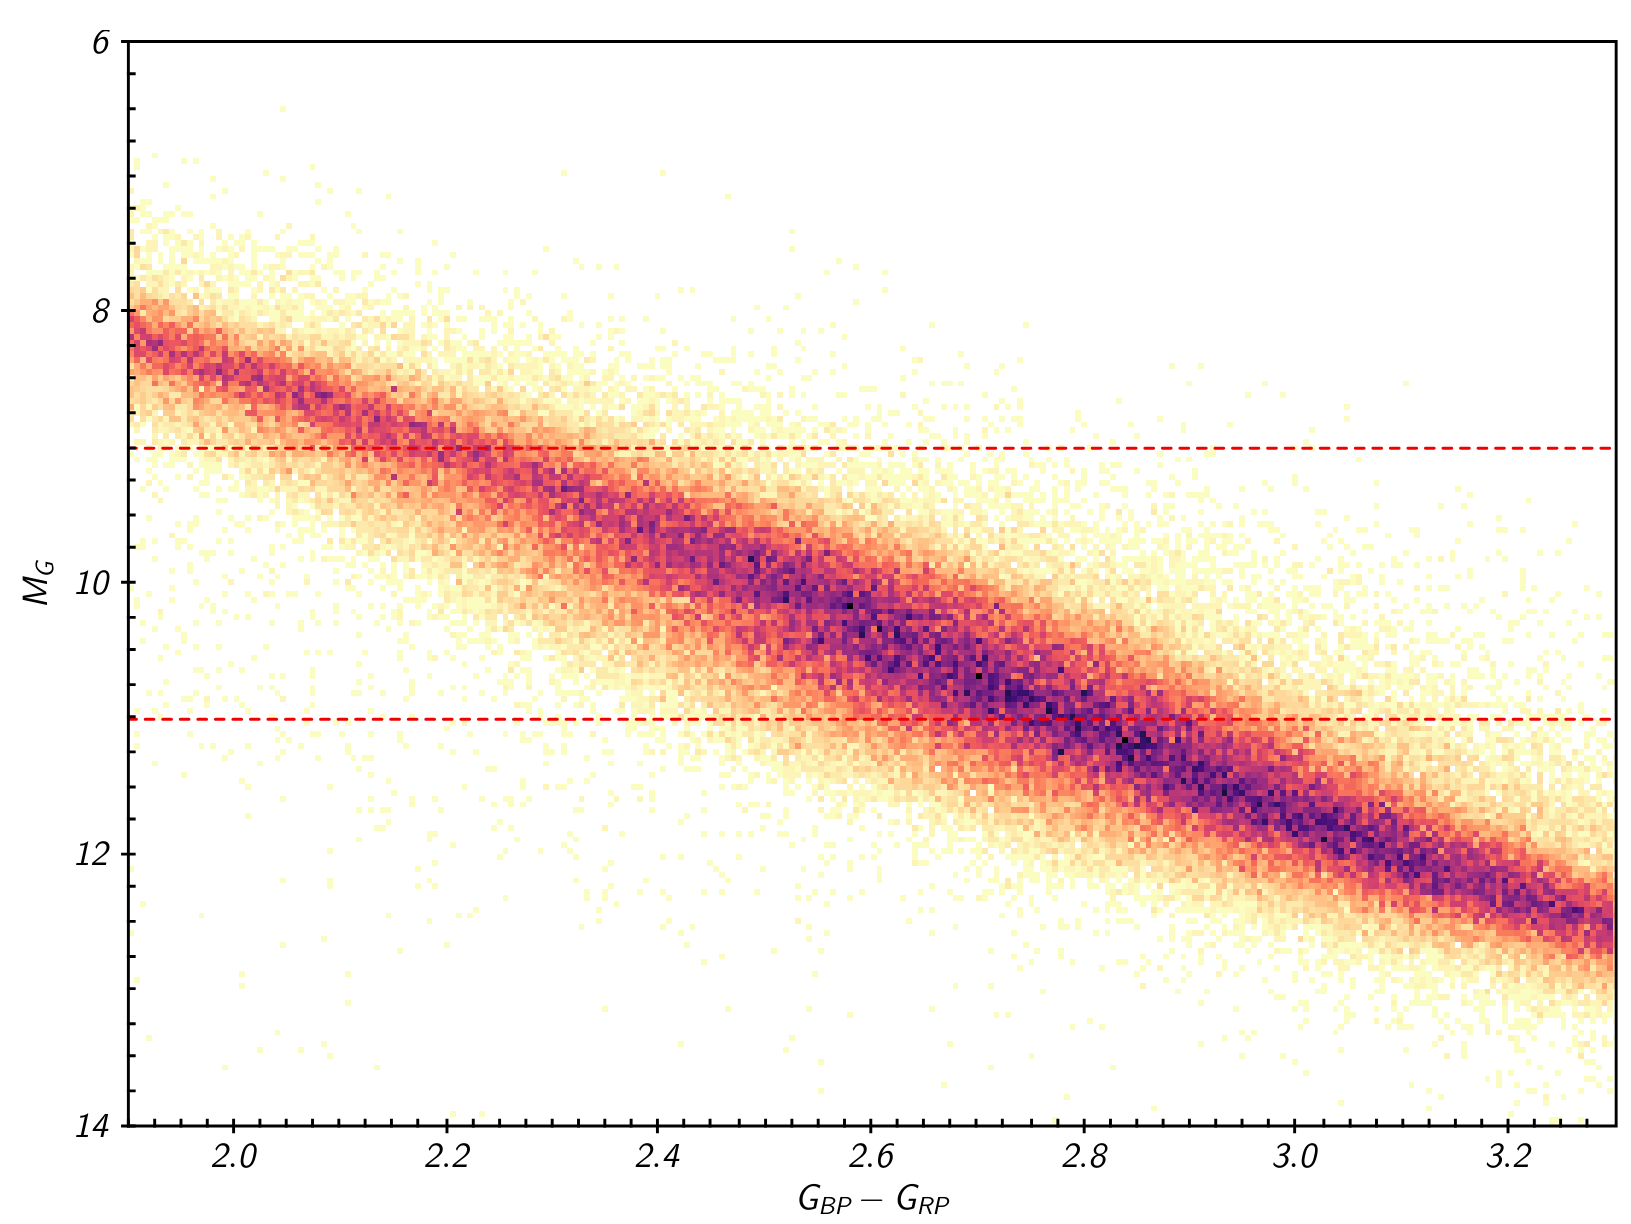
\includegraphics[width=0.45\textwidth]{src/figures/JaoGap.png}
	\caption{Figure 1 from \citet{Jao2018} showing the so called ``Jao Gap'' at
	$M_{G}\approx$ 10 {\color{red} [SHOULD I REMAKE THIS USING DR3 DATA?]}}
	\label{fig:JaoGap}
\end{figure}

The proton-proton I chain constitutes three reactions 
\begin{enumerate} 
	\item $p + p \longrightarrow d + e^{+} + \nu_{e}$
	\item $p + d \longrightarrow \ ^{3}\text{He} + \gamma$
	\item $^{3}\text{He} + ^{3}\text{He} \longrightarrow \ ^{3}\text{He} + 2p$ 
\end{enumerate} 
Because reaction 3 of ppI consumes $^{3}$He at a slower rate than it is
produced by reaction 2, core $^{3}$He abundance, and consequently the rate of
reaction 3, increases with time. The core convective zone expands as more of
the star becomes unstable to convection. This expansion continues until the
core connects with the convective envelope. At this point convective mixing can
transport material throughout the entire of the star and the high concentration
of $^{3}$He rapidly diffuses outward, away from the core, decreasing energy
generation as reaction 3 slows down. Ultimately, this leads to the convective
region around the core pulling back away from the convective envelope, leaving
in place the radiative transition zone, at which point $^{3}$He concentrations
grow in the core until it once again expands to meet the envelope.  These
periodic mixing events will contine until the $^{3}He$ concentration throughout
the star reach an equlibtium ultimatly resulting in a fully convective star.
Figure \ref{fig:Kippenhan1} traces the evolution of a charecteristic star
within the Jao Gap's mass range.

\begin{figure*}
	\centering
	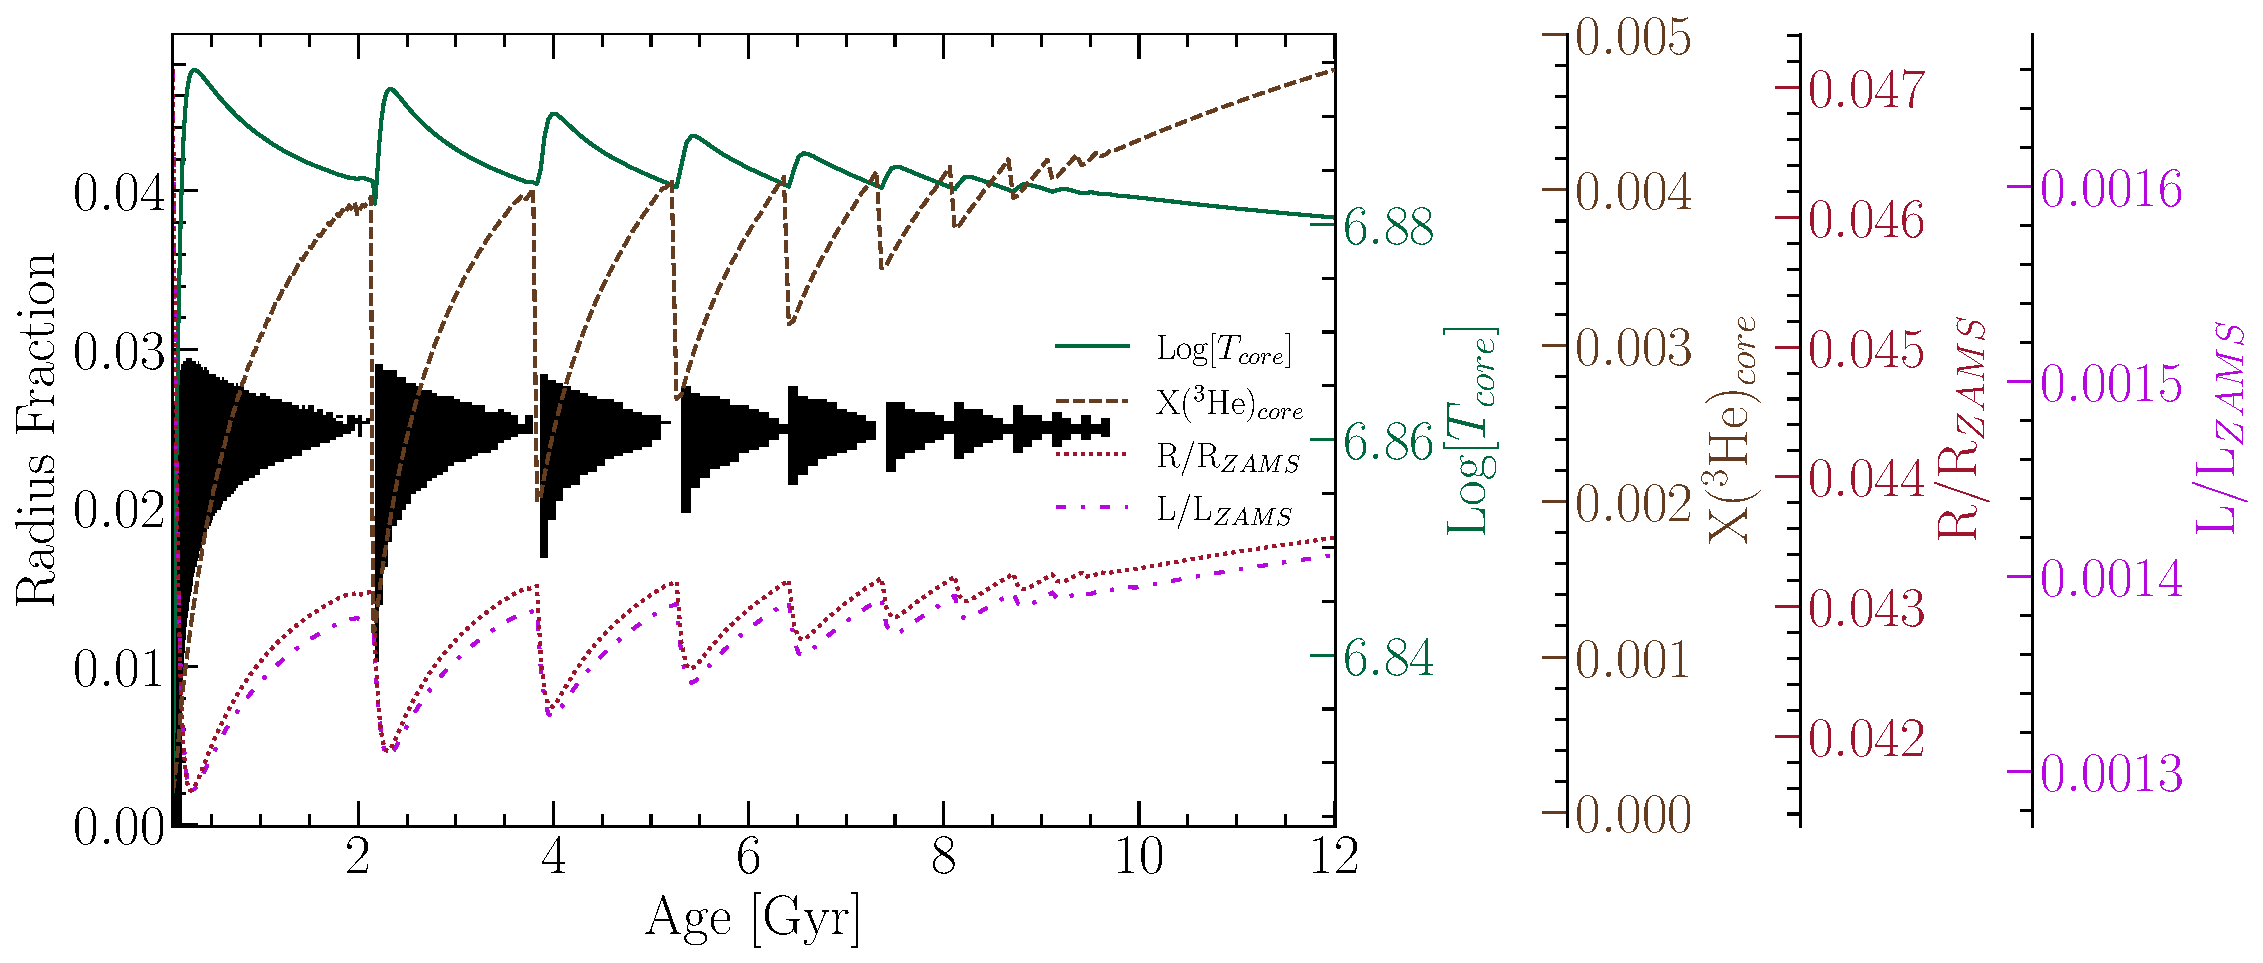
\includegraphics[width=0.95\textwidth]{src/figures/NotebookFigs/Kippenhan.pdf}
	\caption{Kippenhan diagram for a charectaristic stellar model of 0.35625
	$M_{\odot}$ which is within the Jao Gap's mass range. The black shaded
	regions denote whether, at a particular model age, a radial shell within
	the model is radiative or convective (with white meaning convective and
	black meaning radiative). The lines trace the models cote temperature, core
	$^{3}$He mass fraction, fractional luminosity wrt the zero age main
	sequence and fractional radius wrt. the zero age main sequence.}
	\label{fig:Kippenhan1}
\end{figure*}


\subsection{Modeling the Gap}
Since the identification of the Gaia M-dwarf gap, stellar modeling has been
conducted to better constrain its location, effects, and exact cause.
Both \citet{Mansfield2021} and \citet{Feiden2021} identify that the gap's mass
location is correlated with model metallicity --- the mass-luminosity
discontinuity in lower metallicity models being at a commensurately lower mass.
\citet{Feiden2021} suggests this dependence is due to the steep relation of
the radiative temperature gradient, $\nabla_{rad}$, on temperature and in turn,
on stellar mass.

\begin{align}\label{eqn:radGrad}
	\nabla_{rad} \propto \frac{L\kappa}{T^{4}}
\end{align}

As metallicity decreases so does opacity, which, by Equation \ref{eqn:radGrad},
dramatically lowers the temperature where radiation will dominate energy transport
\citep{Chabrier1997}. Since main sequence stars are virialized the core
temperature is proportional to the core density and total mass (Equation
\ref{eqn:TMRelation}). Therefore, if the core temperature where
convective-kissing instability is expected decreases with metallicity, so too
will the mass of stars which experience such instabilities.

\begin{align}\label{eqn:TMRelation}
	T_{c} \propto \rho_{c}M^{2}
\end{align}

This strong opacity dependence presents a slight problem where modeling is 
concerned. With current computational tools it is infeasible to compute opacities on the
fly; rather, Rossland Mean opacity ($\kappa_{R}$) for individual elements must
be pre-tabulated over a wide range of temperatures and densities. These
opacities can then be somewhat arbitrarily mixed together and interpolated to
form opacity lookup-tables. Multiple groups have performed these calculations
and subsequently made tables available to the wider community, these include
the Opacity Project \citep[OP][]{Seaton1994}, Laurence Livermore National Labs
OPAL opacity tables \citep{Iglesias1996}, and Los Alamos National Labs OPLIB
opacity tables \citep{Colgan2016}.


\section{Opacities}\label{sec:opac}
Radiative opacity is fundamental to stellar structure, it determines how much
incident radiation is absorbed or scattered. Moreover, when a media is in
thermodynamic equilibrium with the radiation field, that is when the temperature
of the media and that of the radiation field is the same, the opacity may be
used via Kirchhoff's law to find the emissivity of a material
\citep{Huebner2014}. Local Thermodynamic Equilibrium (LTE) is a common state to
find within a star and therefore stellar models have long relied on opacities
calculated in LTE.

\subsection{OPLIB Opacities}
Los Alamos National Labs OPLIB opacity tables were first computed in the 1990s
using the LEDCOP code \citep{Magee1995}; however, since 2004 efforts have been
underway to shift OPLIP from LEDCOP to ATOMIC \citep{Magee2004}. ATOMIC is a
LTE and non-LTE opacity and plasma modeling code. A major strength of ATOMIC
when compared to the older LEDCOP is its ability to vary its refinement level
\citep{Fontes2016}. For a more detailed breakdown of how the most up-to-date
set of OPLIB tables are generated see \citep{Colgan2016}.

The most up to date OPLIB tables include monochromatic Rosseland mean opacities
for elements hydrogen through zinc over temperatures 0.5eV to 100 keV and for
mass densities from approximately $10^{-8}$ g cm$^{-3}$ up to approximately
$10^{4}$ g cm$^{-3}$ (though the exact mass density range varies as a function
of temperature). The Rosseland mean opacity as reported in OPLIB tables is given
in Equation \ref{eqn:RMOATOMIC}.

\begin{align}\label{eqn:RMOATOMIC}
	\frac{1}{\kappa_{R}} =
		\frac{\int_{0}^{\infty}\frac{1}{\kappa_{\nu}}n_{\nu}^{3}\frac{\partial
		B_{\nu}}{\partial T}d\nu}{\int_{0}^{\infty}\frac{\partial B_{\nu}}{\partial
		T}d\nu}
\end{align}
Here, $B_{\nu}$ is the Planck function, $n_{\nu}$ is the frequency-dependent
refractive index \citep{Armstrong2014}, and $\kappa_{\nu}$ is the
frequency-dependent opacity. $\kappa_{\nu}$ is defined as the sum of the
bound-bound, bound-free, free-free, and scattering opacity computed by ATOMIC.

\subsection{Table Querying and Conversion}
DSEP uses pre-computed high-temperature opacity tables, in the format supplied
by OPAL. These tables list the Rosseland-mean opacity, $\kappa_{R}$, along
three dimensions: temperature, a density proxy R, and composition. R is defined
as
\begin{align} \label{eqn:Req}
	R = \frac{\rho}{T_{6}^{3}}
\end{align}
Where $T_{6} = T\times10^{-6}$ and $\rho$ is the mass density. If $T$ and
$\rho$ are given in cgs then for much of the radius of a star
$\log(R)\sim-1.5$.  The reason DSEP uses $R$ as opposed to simply tracking
opacity over density is that $R$ stays relatively fixed, whereas there is an
enormous dynamic range of densities within a star ($\sim 10^{5}$ [g cm$^{-3}$]
at the core of an RGB star all the way down to $\sim 10^{-8}$ [g
cm$^{-3}$] within the envelope). This reduction in
dynamic-range is important to help reduce floating-point numeric errors, which
ends up being the primary motivation to use $R$ over $\rho$.

OPLIB high-temperature opacity tables will replace the OPAL tables DSEP has used
since the release of the Dartmouth Stellar Evolution Database (DSED) in 2008
\citep{Dotter2008}. Just as OPAL tables were, OPLIB tables are queried from a
web interface\footnote{https://aphysics2.lanl.gov/apps/}. So that we might
generate many tables easily and quickly we develope a web scraper built with
Python's \texttt{requests} module in addition to the 3rd party
\texttt{mechanize} and \texttt{BeautifulSoup} modules \citep{chandra2015python,
richardson2007beautiful} which can get tables with minimal human intervention.
This web scraper submits a user requested chemical composition (composed of
mass fractions for elements from Hydrogen to Zinc) to the Los Alamos web form, selects
0.0005 keV as the lower temperature bound and 60 keV as the upper temperature
bound, and finally requests opacity measurements for 100 densities, ranging
from $1.77827941\times 10 ^{-15}$ [g cm$^{-3}$] up to $1\times10^{7}$ [g
cm$^{-3}$], at each temperature interval. These correspond to approximately the
same temperature and density range of opacities present in the OPAL opacity
tables.

So as not to break compatibility with OPAL tables we create a translation layer
to convert OPLIB tables to OPAL format. This allows for transparent use of the new
tables without any direct modifications to the DSEP source. The primary job of
this translation layer is to unit conversion, secondarily the structure of OPAL
tables must be matched byte-for-byte.

OPLIB reports $\kappa_{R}$ as a function of mass density, temperature in keV,
and composition. Recall that OPAL tables present opacity as a function of
temperature in Kelvin, $R$, and composition. The conversion from temperature
in keV to Kelvin is trivial
\begin{align}
	T_{K} = T_{keV} * 11604525.0061657
\end{align}
The conversion from mass density to $R$ is more involved. Because $R$ is
coupled with both mass density and temperature there there is no way to
directly convert tabulated values of opacity reported in the OPLIB tables to
their equivalents in $R$ space. Instead we must rotate the tables,
interpolating $\kappa_{R}(\rho,T_{eff}) \rightarrow \kappa_{R}(R,T_{eff})$. 

As a first step in this rotation we use the \texttt{interp2d} function within
\texttt{scipy}'s \texttt{interpolate} \citep{2020SciPy-NMeth} module to
construct a cubic bivariate B-spline \citep{Dierckx1981} interpolating function
$s$, with a smoothing factor of 0, representing the surface $\kappa_{R}(\rho,
T_{eff})$. For each $R^{i}$ and $T^{j}_{eff}$ which DSEP expects
high-temperature opacities to be reported for, we evaluate Equation
\ref{eqn:Req} to find $\rho^{ij} = \rho(T^{j}_{eff},R^{i})$.  Opacities in
$T_{eff}$, $R$ space are then inferred as $\kappa^{ij}_{R}(R^{i},T^{j}_{eff}) =
s(\rho^{ij}, T^{j}_{eff})$. Finally, some number of upper-left and lower-right
hand entries in each table are discarded as DSEP takes non rectangular tables
as input, the exact number and indices of the discarded entries is dependent
on composition.

As first-order validation of this interpolation scheme we can preform a similar
interpolation in the opposite direction, rotating the tables back to
$\kappa_{R}(\rho, T_{eff})$ and then comparing the initial, ``raw'', opacities
to those which have gone through the interpolations process. Figure
\ref{fig:fracdiff} shows the fractional difference between the raw opacities
and a set which have gone through this double interpolation. The red line
denotes $Log(R)=-1.5$ where models will tend to sit for much of their radius.
Along the $Log(R)=-1.5$ line the mean fractional difference is $\langle \delta
\rangle = 0.006$ with an uncertainty of $\sigma_{\langle\delta\rangle} =
0.009$. One point of note is that, because the initial rotation into $Log(R)$
space also reduces the domain of the opacity function interpolation-edge
effects which we avoid initially by extending the domain past what DSEP needs
cannot be avoided when interpolating back into $\rho$ space. In future, a more
robust validation, which does not reduce the domain size will be conducted.

\begin{figure}
	\centering
	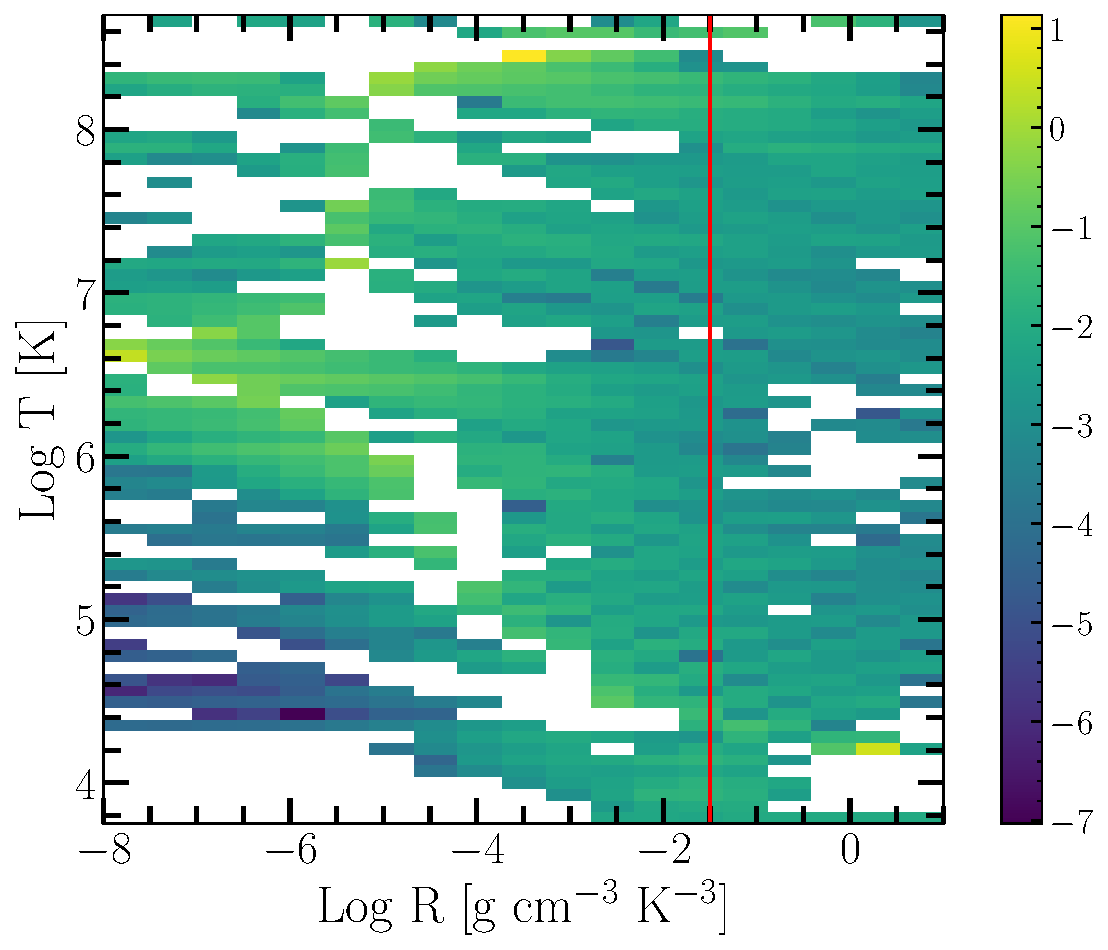
\includegraphics[width=0.45\textwidth]{src/figures/FractionalDifference.pdf}
	\caption{Log Fractional Difference between opacities in $\kappa_{R}(\rho,
	T_{eff})$ space directly queried from the OPLIB webform and those which
	have been interpolated into $Log(R)$ space and back. Note that, due to the
	temperature grid DSEP uses not aligning perfectly which the temperature
	grid OPLIB uses there may be edge effects where the interpolation is poorly
	constrained. The red line corresponds to $Log(R) = -1.5$ where much of a
	stellar model's radius exists.}
	\label{fig:fracdiff}
\end{figure}

\subsection{Opacity Validation}
In order to further validate the OPLIB high-temperature opacities we first visually
compare a set of opacity vs. temperature curves from OPLIB at a constant $R$
and \citet{Grevesse1998} composition (GS98) to the same curve from OPAL. A
characteristic opacity vs temperature curve is shown in Figure
\ref{fig:OpacCompare}, $\log _{10}(R) = -1.5$ is chosen as for much of the
radius of a main sequence star $\log _{10}(R)$ is around that value. The
largest variation in $\kappa_{R}$ from OPAL to OPLIB at $\log _{10}(R)=-1.5$ is
on the order of a few percent. This is inline with expectations of OPLIB and OPAL
being in relatively close agreement \citep{Colgan2016}.

\begin{figure}
	\centering
	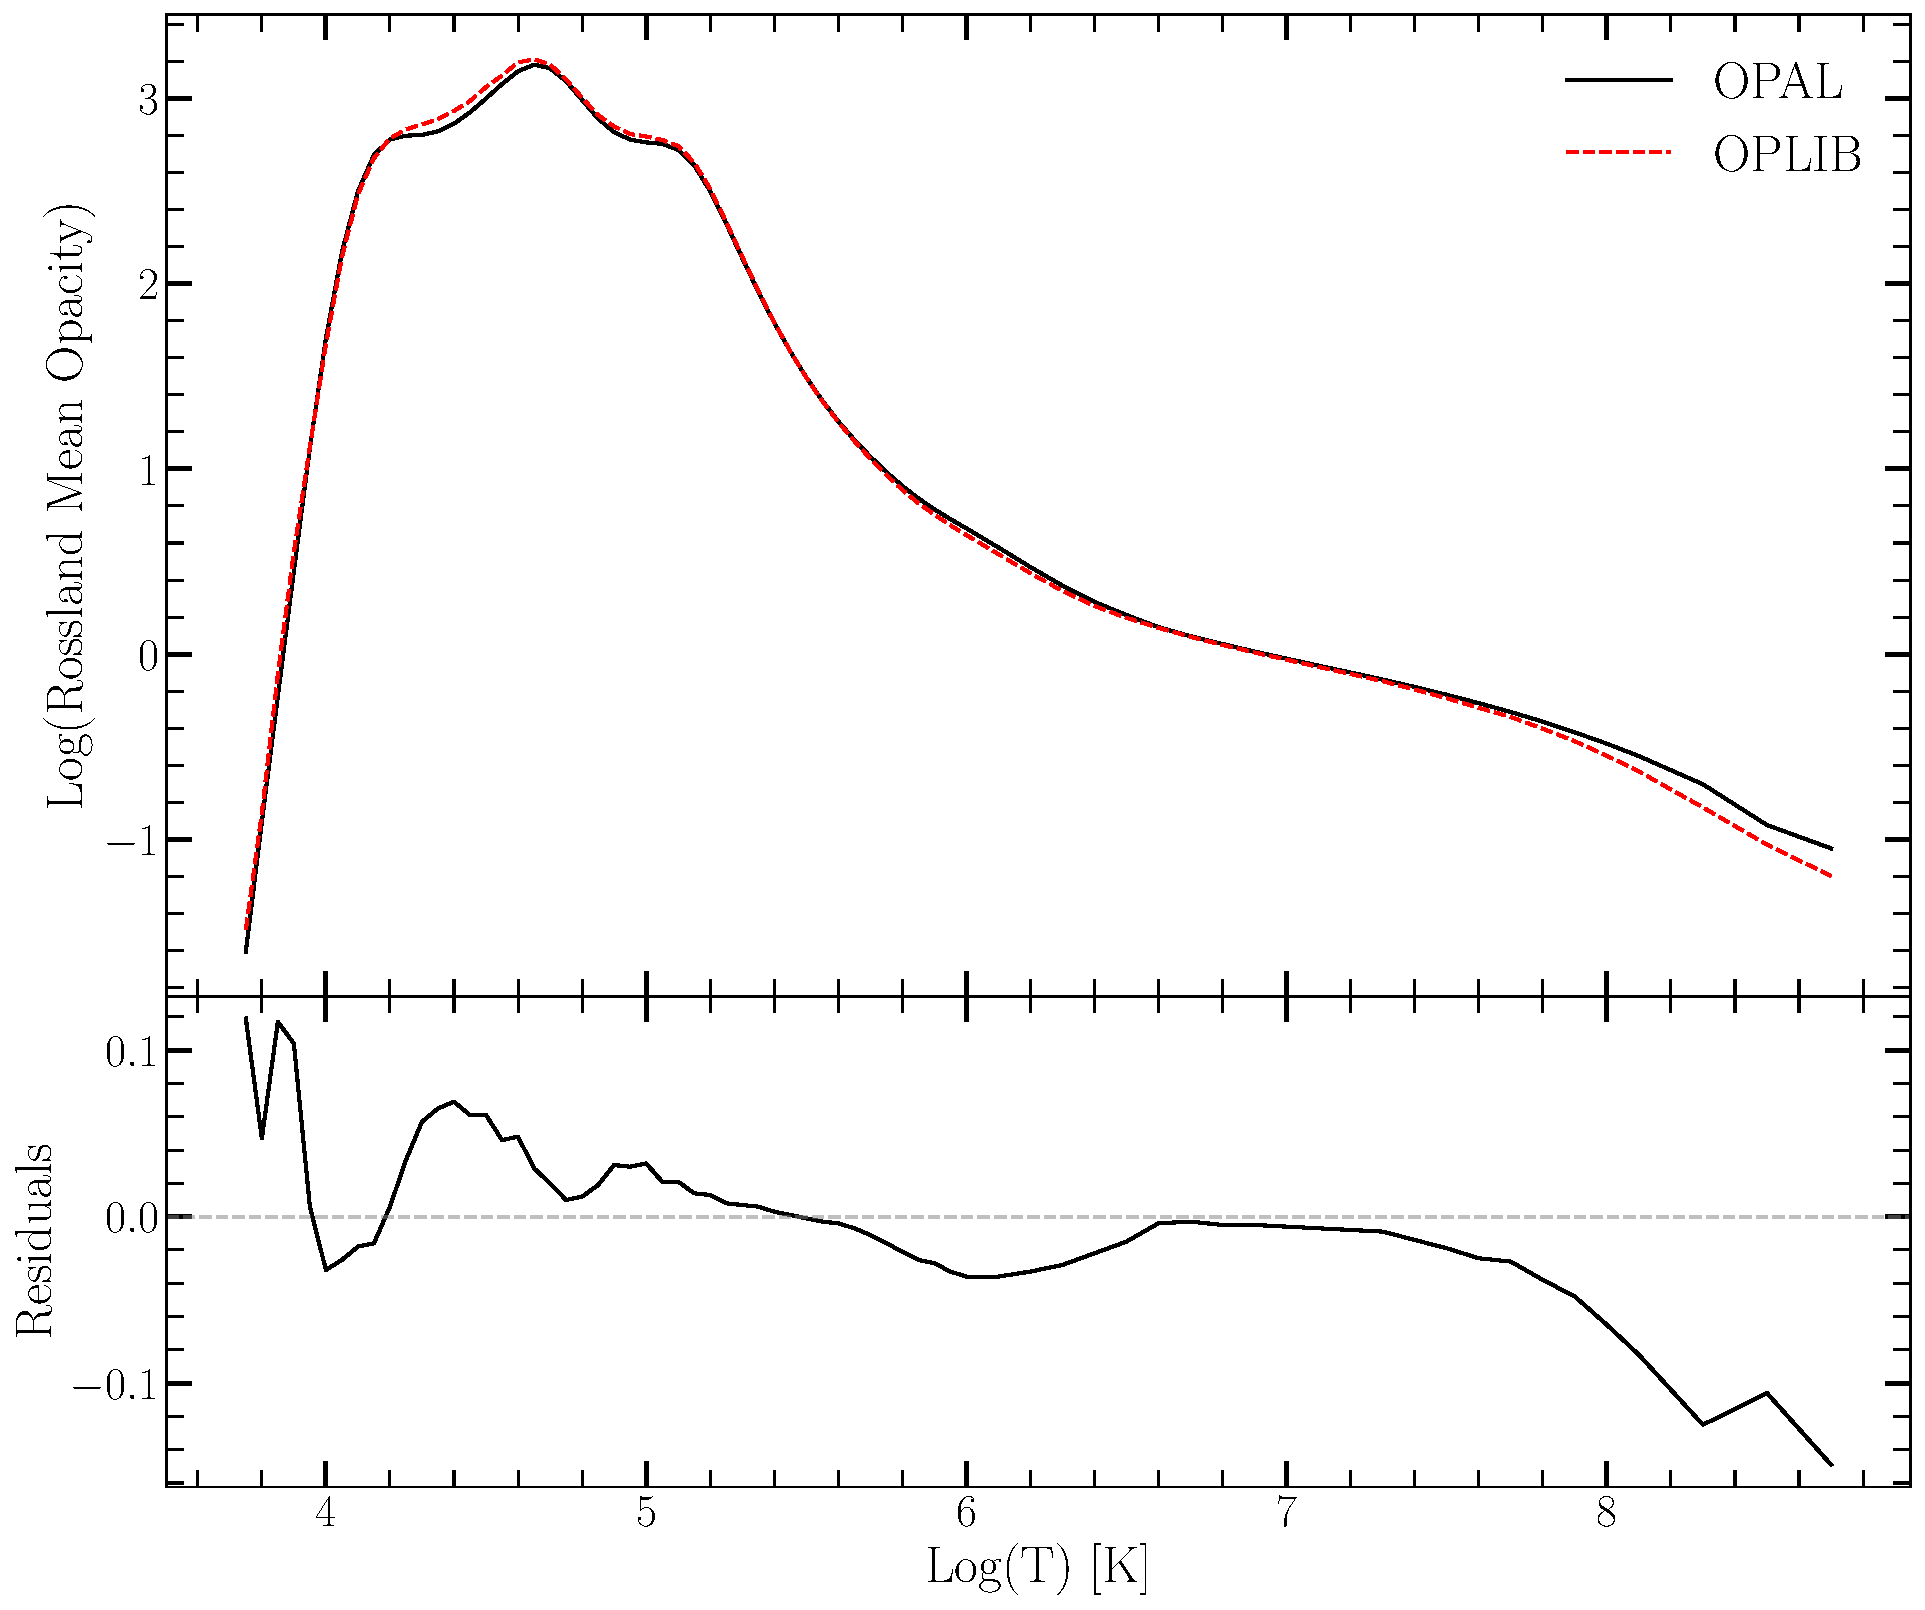
\includegraphics[width=0.45\textwidth]{src/figures/OpacityComparision.pdf}
	\caption{Rosseland mean opacity with the GS98 solar composition for both
		OPAL opacities and OPLIB opacities (top). Residuals between OPLIB
		opacities and OPAL opacities (bottom). These opacities are plotted at
		$\log _{10}(R) = -1.5$, $X=0.7$, and $Z=0.02$.}
	\label{fig:OpacCompare}
\end{figure}

To further validate the OPLIB opacities we generate a solar calibrated stellar
model (SCSM) using the new tables. SCSMs are generally models where some
initial parameters have been iteratively adjusted to minimize some loss function
between that models output parameters and the observed values of those
parameters for the Sun. In the context of this paper we adjust both the
convective mixing length parameter, $\alpha_{ML}$, and the initial Hydrogen
mass fraction, $X$, to minimize the difference between the models final radius
and luminosity and that of the sun.

Optimization of $\alpha_{ML}$ and $X$ is done with a quite naive gradient
descent algorithm. For each optimization step three models are evolved: a reference
model, a model with a small perturbation to the hydrogen mass fraction but the
same mixing length as the reference model, and a model with a small
perturbation to the mixing length but the same hydrogen mass fraction as the
reference. Perturbations are sampled from a normal distribution (implemented
though \texttt{numpy.random}) with scale set to an adjustable parameter,
$\eta$. This distribution is sampled and that sample is then added to the
reference value for either $X$ or $\alpha_{ML}$. The luminosity and radius of
the three evolved models are compared to solar values and the gradient of the
resultant $L-L_{\odot}$, $R-R_{\odot}$ surface is followed down to new
estimates for the reference values of $X$ and $\alpha_{ML}$. This process is
is repeated until the difference between successive $X$ and $\alpha_{ML}$ drops
below one part in $10^{5}$.

\begin{figure}
	\centering
	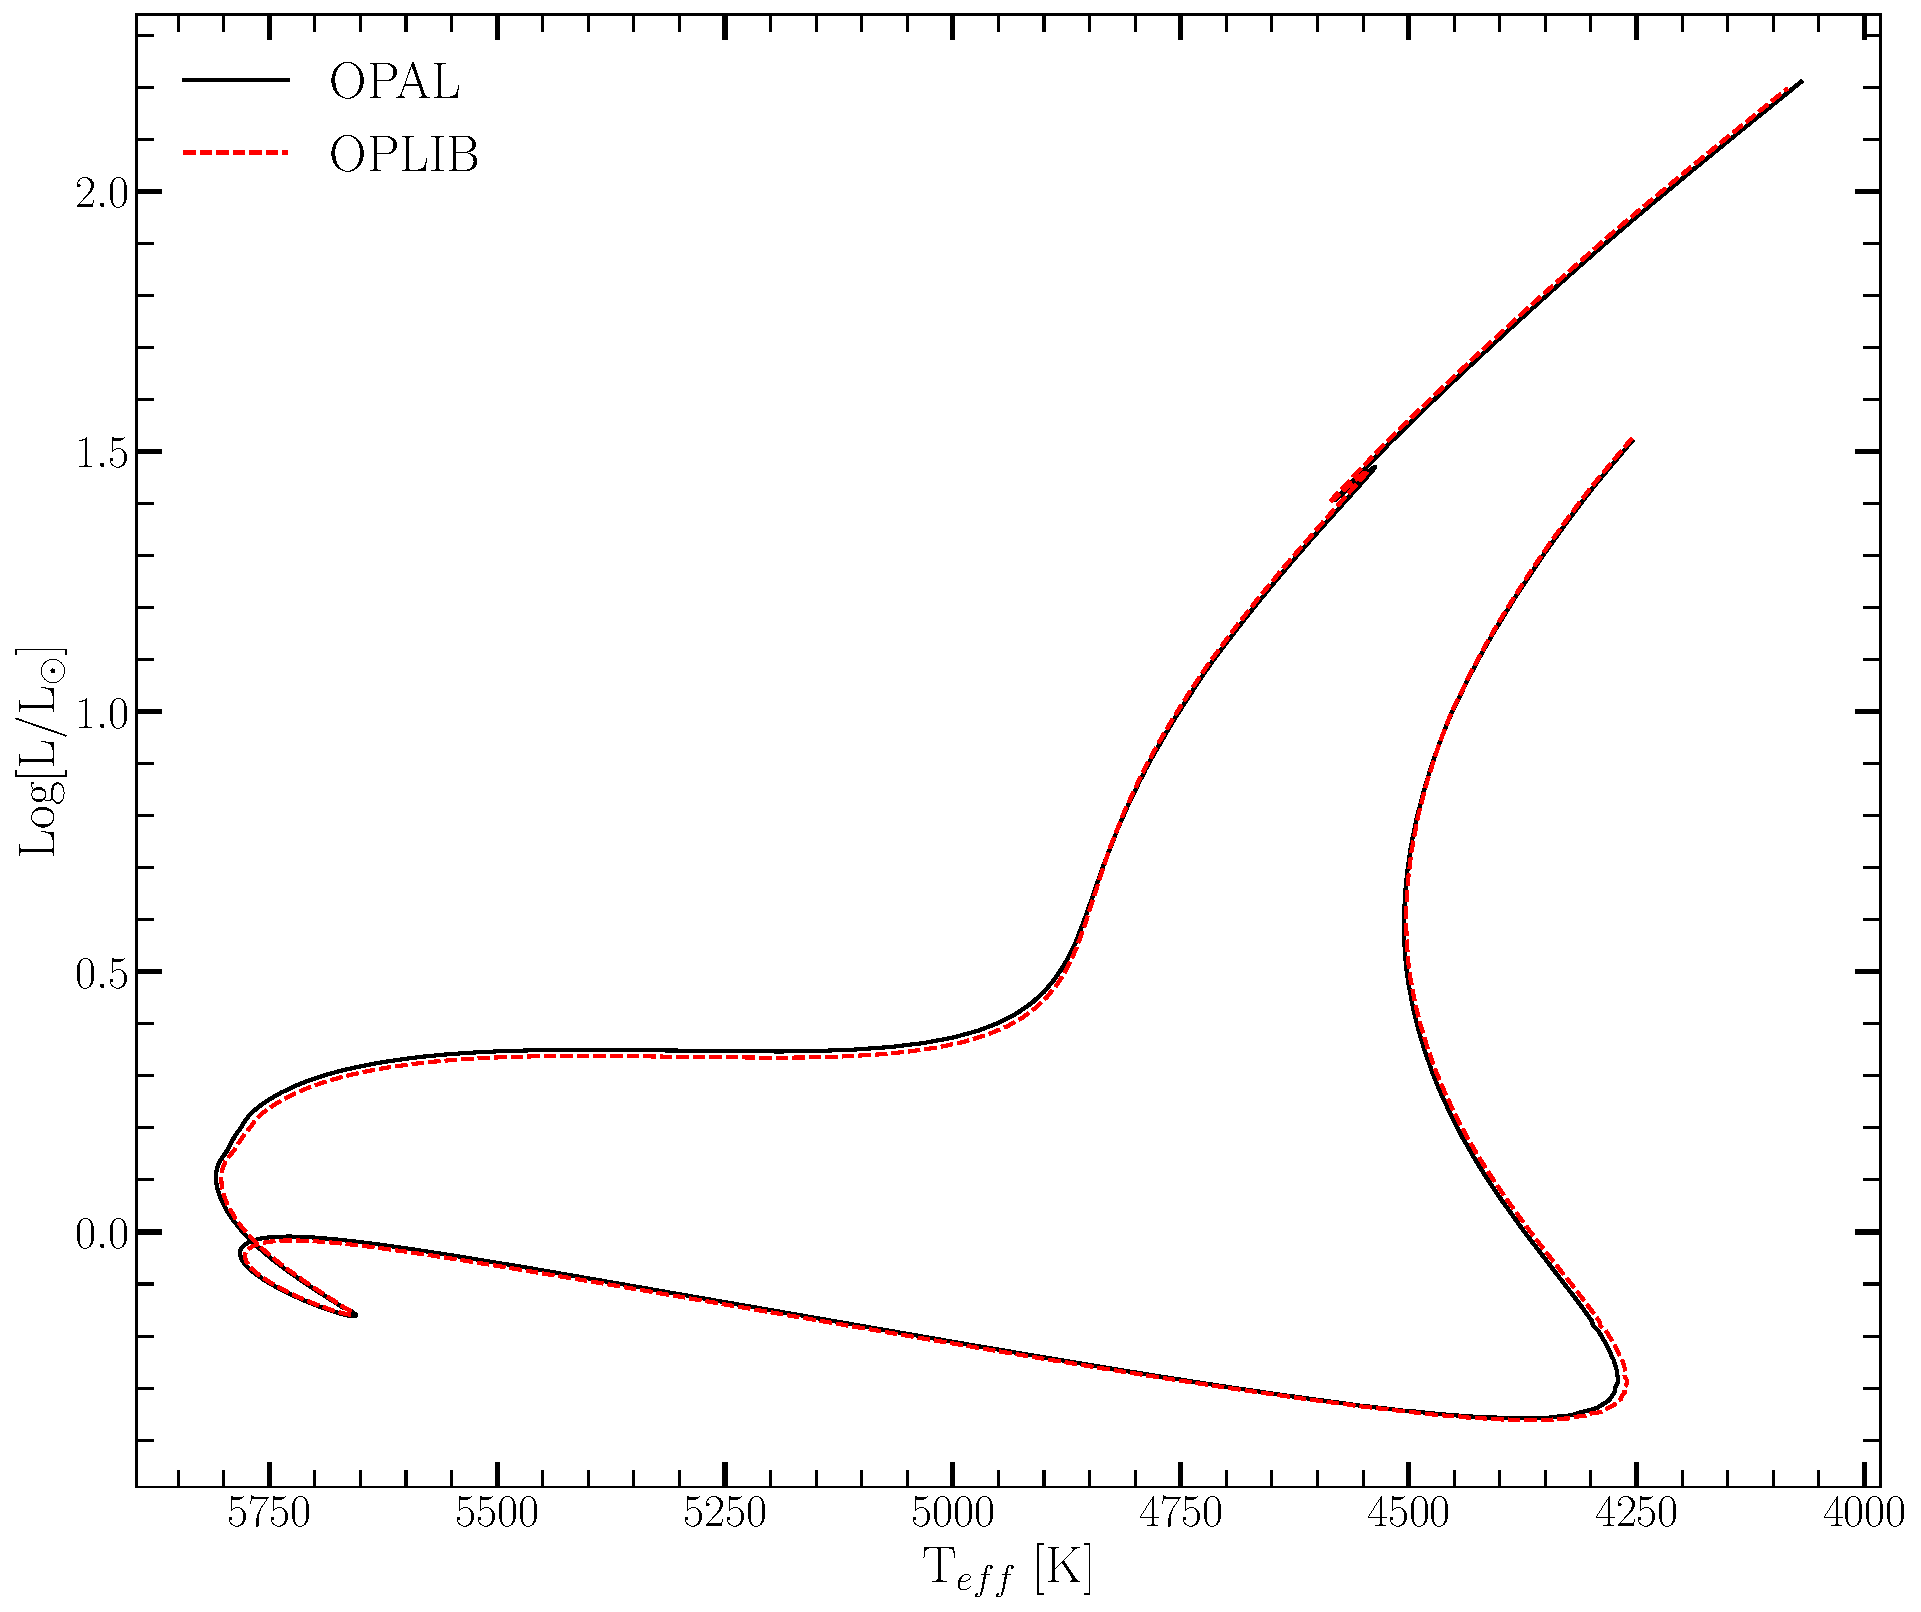
\includegraphics[width=0.45\textwidth]{src/figures/HRDiagramOPALvsOPLIB_SCCM.pdf}
	\caption{HR Diagram for the two SCSMs, OPAL and OPLIB. OPLIB is show as a grey
	dashed line.}
	\label{fig:OPLIBOPALHR}
\end{figure}

If we generate a SCSM using the GS98 OPAL opacity tables we find a best
estimate of $X=0.7066$ and $\alpha_{ML} = 1.9333$. When we preform the same
calibration but substituting in the GS98 OPLIB tables we find $X=0.7107$ and
$\alpha_{ML} = 1.9629$. This represents $\sim 0.5\%$ difference in the SCSM
hydrogen mass fractions and $\sim 1.5\%$ change in the SCSM convective mixing
length parameters when comparing models using OPAL and OPLIB tables. An
HR-diagram for the two calibrated models is presented in Figure
\ref{fig:OPLIBOPALHR}. While the two evolutionary tracks are very similar, note
that the OPLIB SCSM's luminosity is systematically lower at the same effective
temperature all the way from the premain sequence up and until the star leaves
the main sequence, at which point it is effectively the same as the OPAL SCSM.
This luminosity difference between OPAL and OPLIB based models is consistent
with expectations given the differences in opacities. Opacity is of primary
importance only in radiative regions of a star ($\gtrsim 10^{6}$ K). Figure
\ref{fig:OpacCompare} shows that OPLIB opacities are uniformly lower than OPAL
opacities above $10^{6}$ K. These lower opacities will steepen the temperature
gradient within the stellar model as radiation streams more freely outward.


\section{Solar Calibrated Stellar Models}\label{sec:SCSM}
% In order to further validate the OPLIB high-temperature opacities we first visually
% compare a set of opacity vs. temperature curves from OPLIB at a constant $R$
% and \citet{Grevesse1998} composition (GS98) to the same curve from OPAL. A
% characteristic opacity vs temperature curve is shown in Figure
% \ref{fig:OpacCompare}, $\log _{10}(R) = -1.5$ is chosen as for much of the
% radius of a main sequence star $\log _{10}(R)$ is around that value. The
% largest variation in $\kappa_{R}$ from OPAL to OPLIB at $\log _{10}(R)=-1.5$ is
% on the order of a few percent. This is inline with expectations of OPLIB and OPAL
% being in relatively close agreement \citep{Colgan2016}.


In order to validate the OPLIB opacities, we generate a solar calibrated
stellar model (SCSM) using these new tables. We allow both the convective
mixing length parameter, $\alpha_{ML}$, and the initial Hydrogen mass fraction,
$X$, to vary simultaneously, minimizing the difference between resultant
models' final radius and luminosity to those of the sun.

Optimization of $\alpha_{ML}$ and $X$ is conducted using gradient descent. For
each optimization step three models are evolved: a reference model, a model
with a small perturbation to the hydrogen mass fraction but the same mixing
length as the reference model, and a model with a small perturbation to the
mixing length but the same hydrogen mass fraction as the reference.
Perturbations are sampled from a normal distribution (using
\texttt{numpy.random}). This distribution is sampled and that sample is then
added to the reference value for either $X$ or $\alpha_{ML}$. The luminosity
and radius of the three evolved models are compared to solar values and the
gradient of the resultant $L-L_{\odot}$, $R-R_{\odot}$ surface is followed down
to new estimates for the reference values of $X$ and $\alpha_{ML}$. This
process is is repeated until the difference between successive $X$ and
$\alpha_{ML}$ drops below one part in $10^{5}$.

\begin{figure}
	\centering
	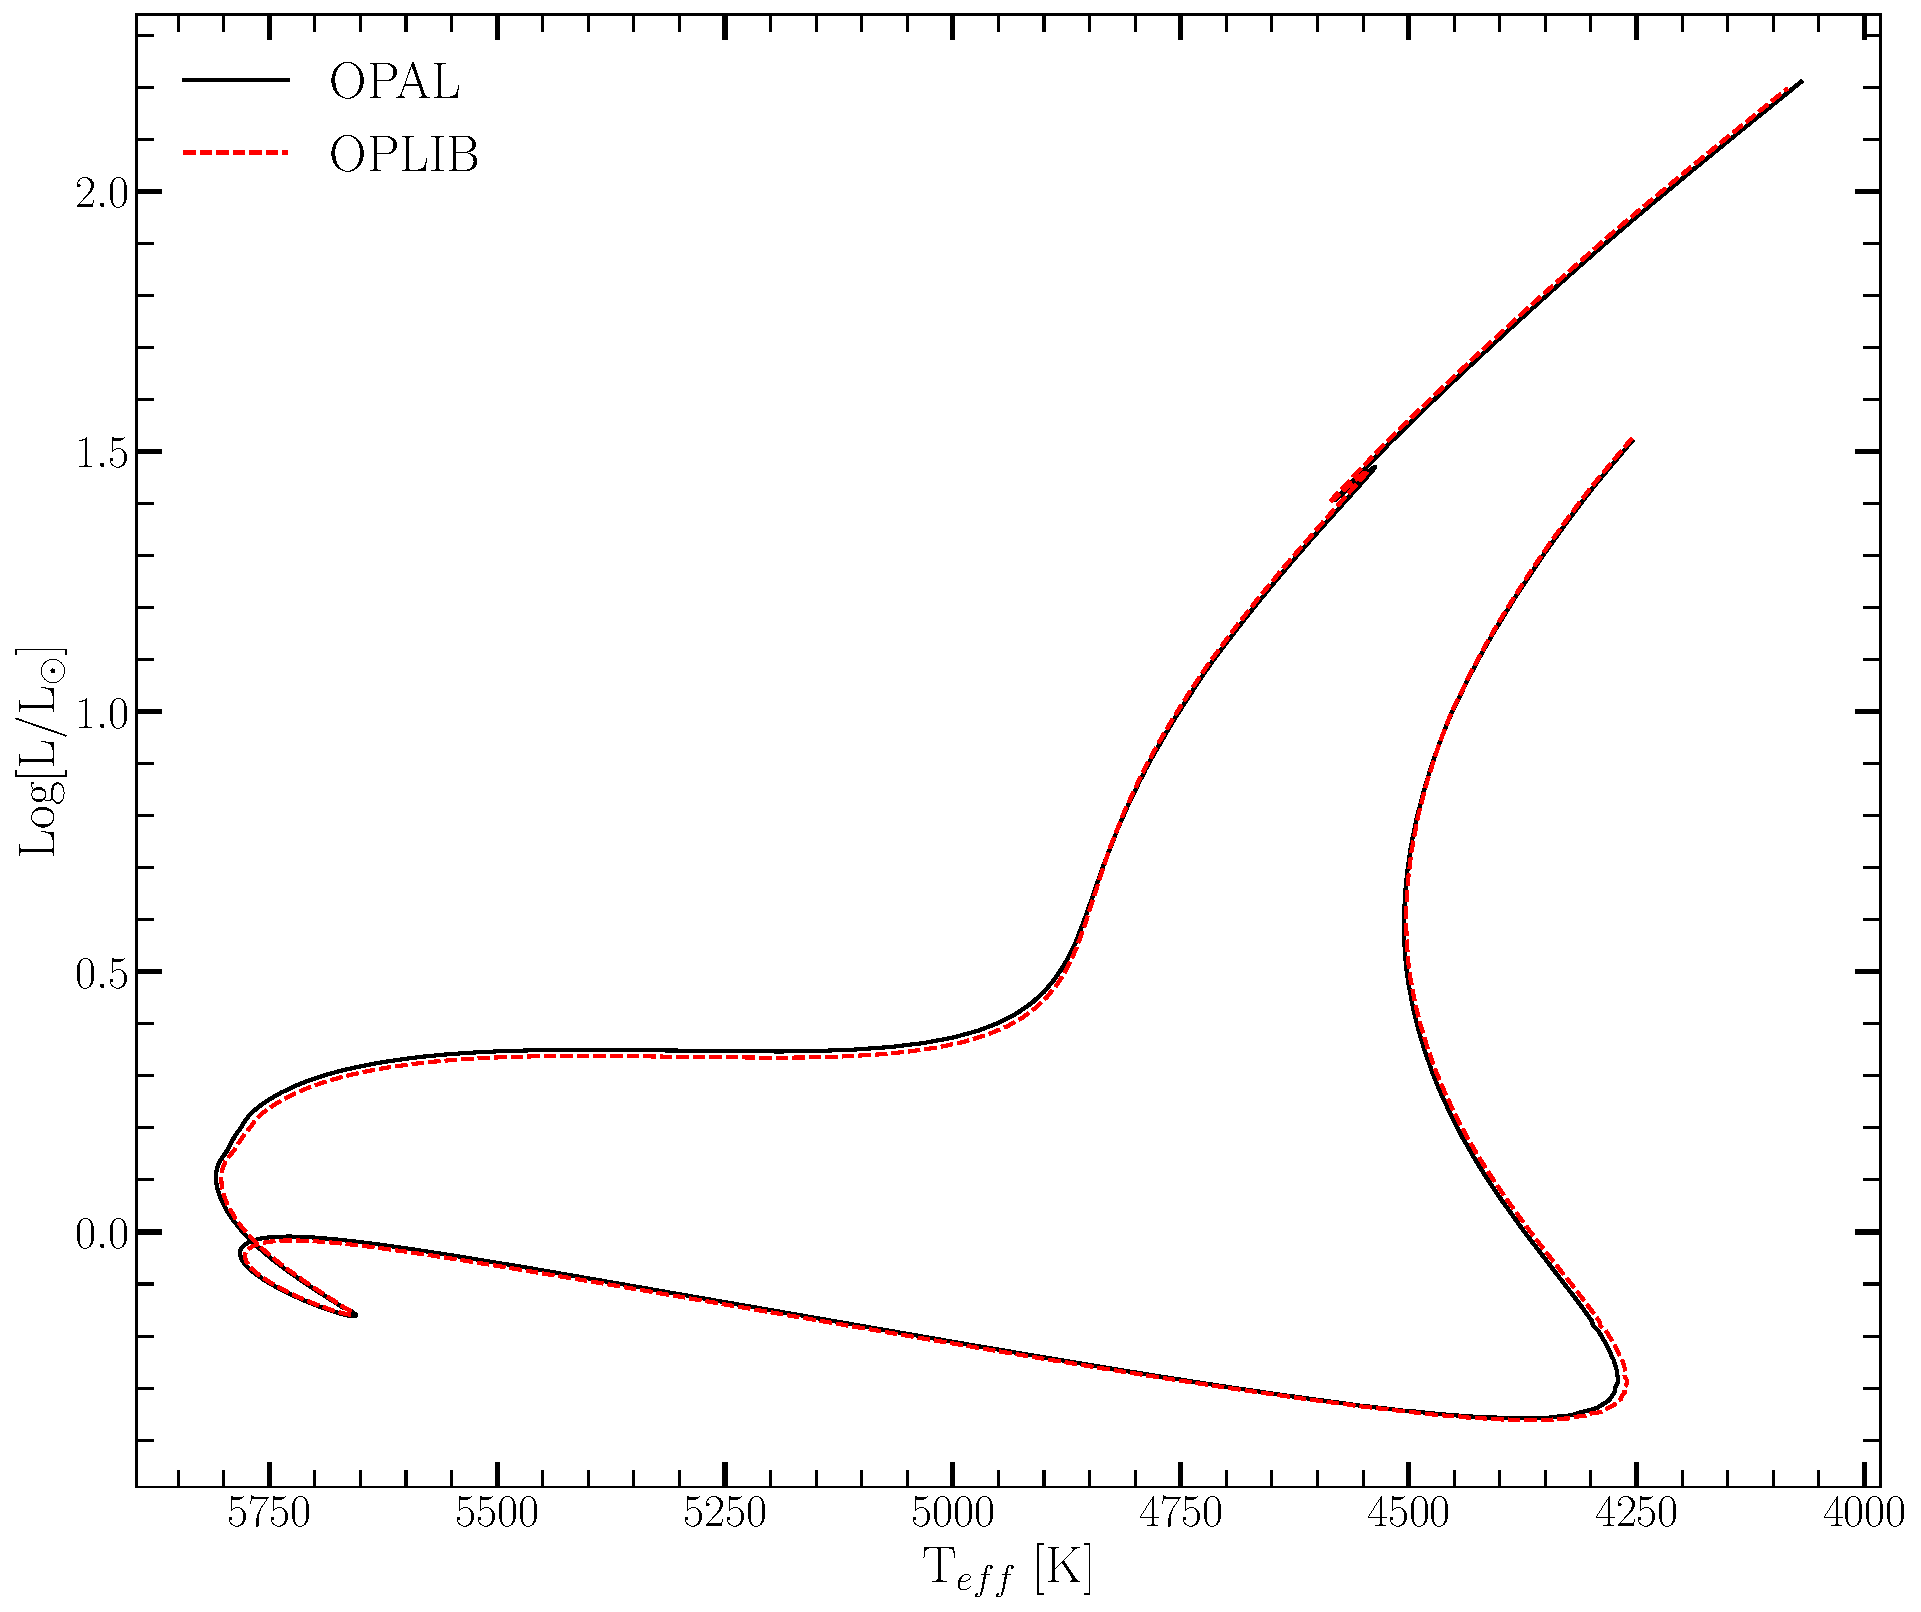
\includegraphics[width=0.45\textwidth]{src/figures/HRDiagramOPALvsOPLIB_SCCM.pdf}
	\caption{HR Diagram for the two SCSMs, OPAL and OPLIB. OPLIB is shown as a grey
	dashed line.}
	\label{fig:OPLIBOPALHR}
\end{figure}

Solar calibrated stellar models evolved using GS98 OPAL and OPLIB opacity
tables (Figure \ref{fig:OPLIBOPALHR}) differ $\sim 0.5\%$ in the SCSM hydrogen
mass fractions and $\sim 1.5\%$ in the SCSM convective mixing length parameters
(Table \ref{tab:SCSMResults}). While the two evolutionary tracks are very
similar, note that the OPLIB SCSM's luminosity is systematically lower at the
same age until the star leaves the main sequence, at which point it is
effectively the same as the OPAL SCSM. This luminosity difference between OPAL
and OPLIB based models is consistent with expectations given the shallow
radiative temperature gradient resulting from the lower OPLIB opacities

\begin{table}
	\centering
	\begin{tabular}{l c c}
		\hline
		Model & $X$ & $\alpha_{ML}$ \\
		\hline
		\hline
		OPAL & 0.7066 & 1.9333 \\
		OPLIB & 0.7107 & 1.9629
	\end{tabular}
	\caption{Optimized parameters for SCSMs evolved using OPAL and OPLIB high
	temperature opacity tables.}
	\label{tab:SCSMResults}
\end{table}


\section{Modeling}\label{sec:modeling}
In order to model the Jao Gap we evolve two extremely finely sampled mass grids
of models. One of these grids uses the OPAL high-temperature opacity tables
while the other uses the OPLIB tables (Figure \ref{fig:PunchIn}). Each grid
evolves a model every 0.00025 $M_{\odot}$ from 0.2 to 0.4 $M_{\odot}$ and every
0.005 $M_{\odot}$ from 0.4 to 0.8 $M_{\odot}$. All models in both grids use a
GS98 solar composition, the (1, 101, 0) \texttt{FreeEOS} (version
{\color{red}2.7}) configuration, and 1000 year old pre-main sequence polytropic
models, with polytropic index 1.5, as their initial conditions.

Because in this work we are just interested in the location shift of the Gap as
the opacity source varies, we do not model variations in composition.
\citet{Mansfield2021,Jao2020,Feiden2021} all look at the effect composition has
on Jao Gap location. They find that as population metallicity increases so too
does the mass range and consequently the magnitude of the Gap. From an extremely
low metallicity population (Z=0.001) to a population with a more solar like
metallicity this shift in mass range can be up to 0.05 M$_{\odot}$
\citep{Mansfield2021}.

\begin{figure}
	\centering
	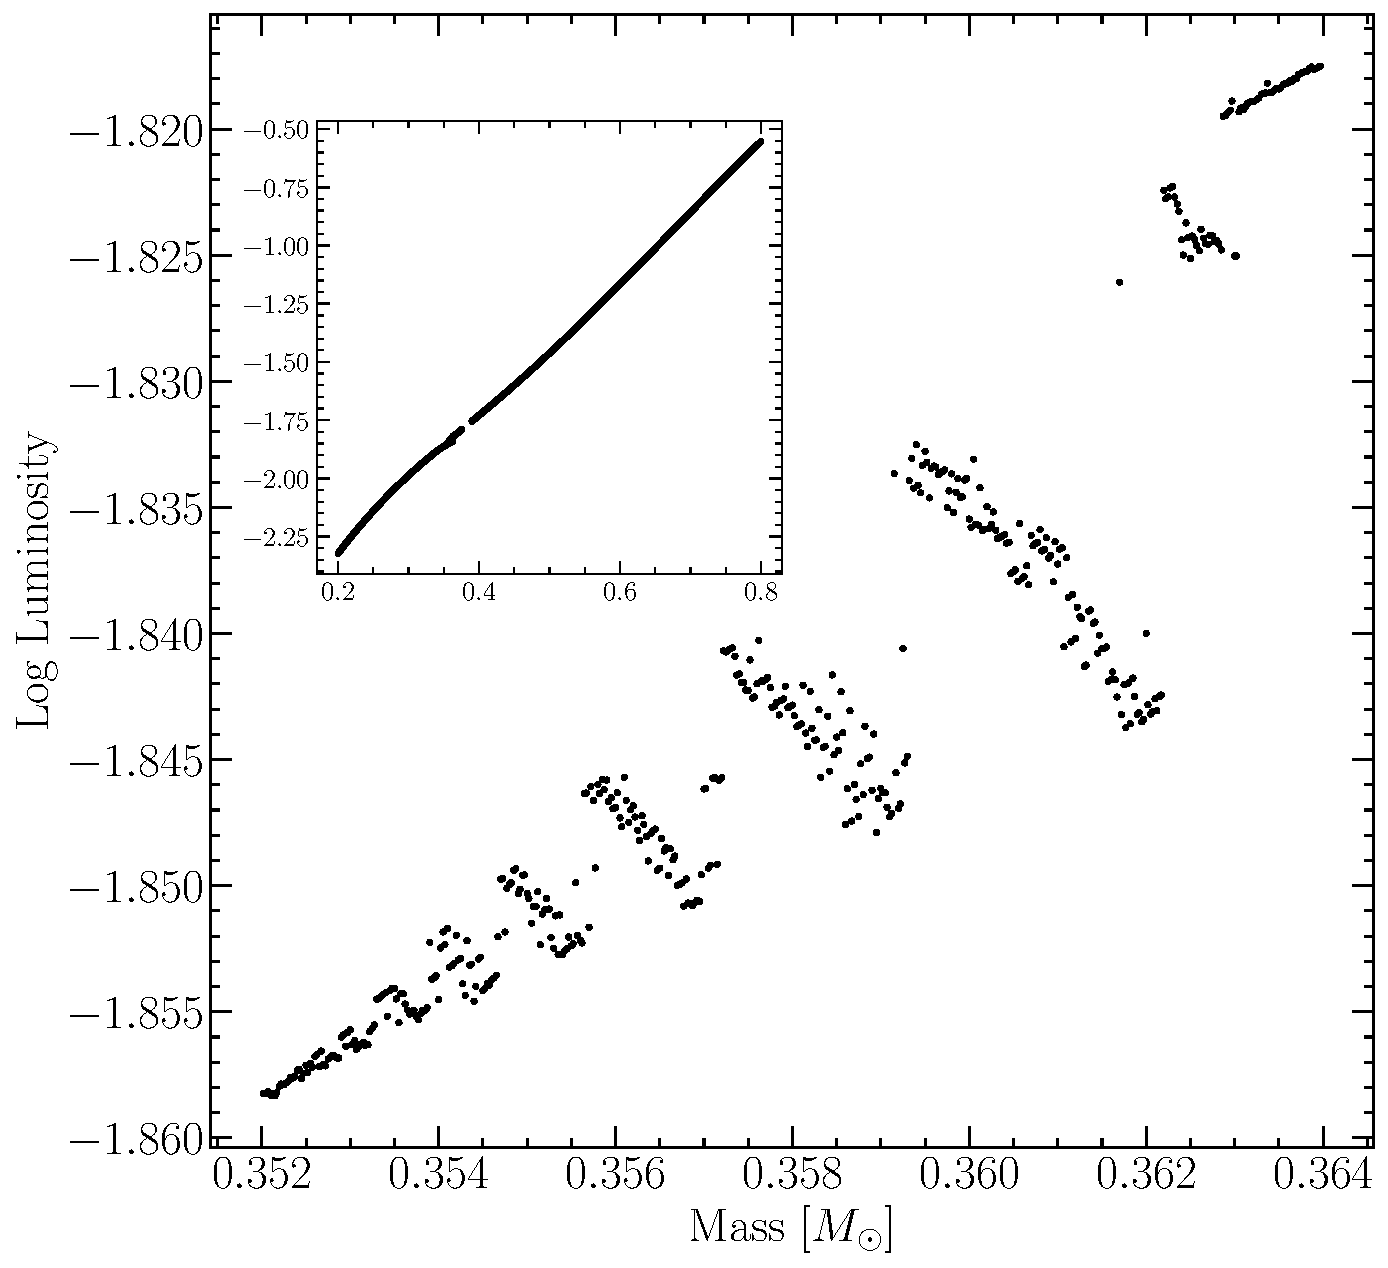
\includegraphics[width=0.45\textwidth]{src/figures/NotebookFigs/OPALPunchIn.pdf}
	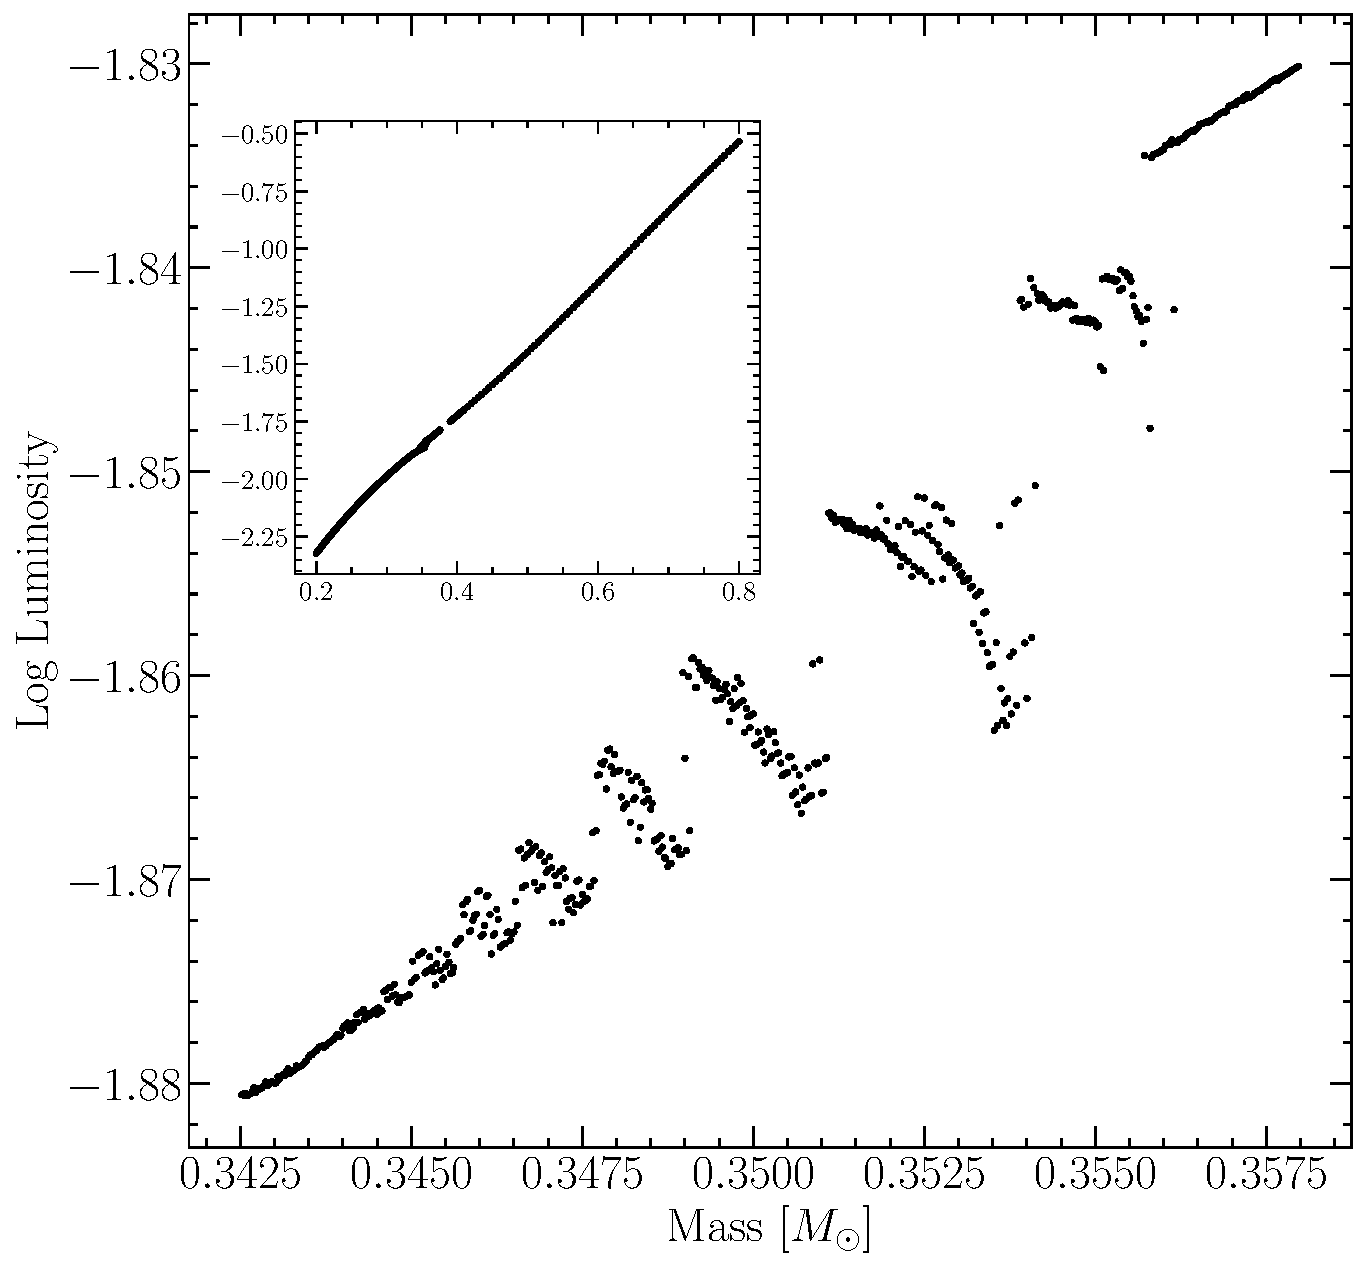
\includegraphics[width=0.45\textwidth]{src/figures/NotebookFigs/OPLIBPunchIn.pdf}
	\caption{Mass-luminosity relation at 7 Gyrs for models evolved using OPAL opacity
	tables (top) and those evolved using OPLIB opacity tables (bottom). Note
	the lower mass range of the OPLIB Gap.}
	\label{fig:PunchIn}
		
\end{figure}

\subsection{Population Synthesis}
In order to compare the Gap to observations we use in house population
synthesis code. We empirically calibrate the relation between G, BP, and RP
magnitudes and their uncertainties along with the parallax/G magnitude
uncertainty relation using the Gaia Catalouge of Nearby Stas
\citep[GCNS,][]{GaiaCollaboration2021} and Equations \ref{eqn:plxCalib} \&
\ref{eqn:MagCalib}. $M_{g}$ is the Gaia G magnitude while $M_{i}$ is the
magnitude in the i$^\text{th}$ band, G, BP, or RP. The coefficients $a$, $b$,
and $c$ determined using a non-linear least squares fitting routine. Equation
\ref{eqn:plxCalib} then models the relation between G magnitude and parallax
uncertainty while Equation \ref{eqn:MagCalib} models the relation between each
magnitude and its uncertainty.

\begin{align}\label{eqn:plxCalib}
	\sigma_{plx}(M_{g}) = ae^{bM_{g}}+c
\end{align}
\begin{align}\label{eqn:MagCalib}
	\sigma_{i}(M_{i}) = ae^{M_{i}-b}+c
\end{align}

\noindent The full series of steps in our population synthesis code
are:

\begin{figure}
	\centering
	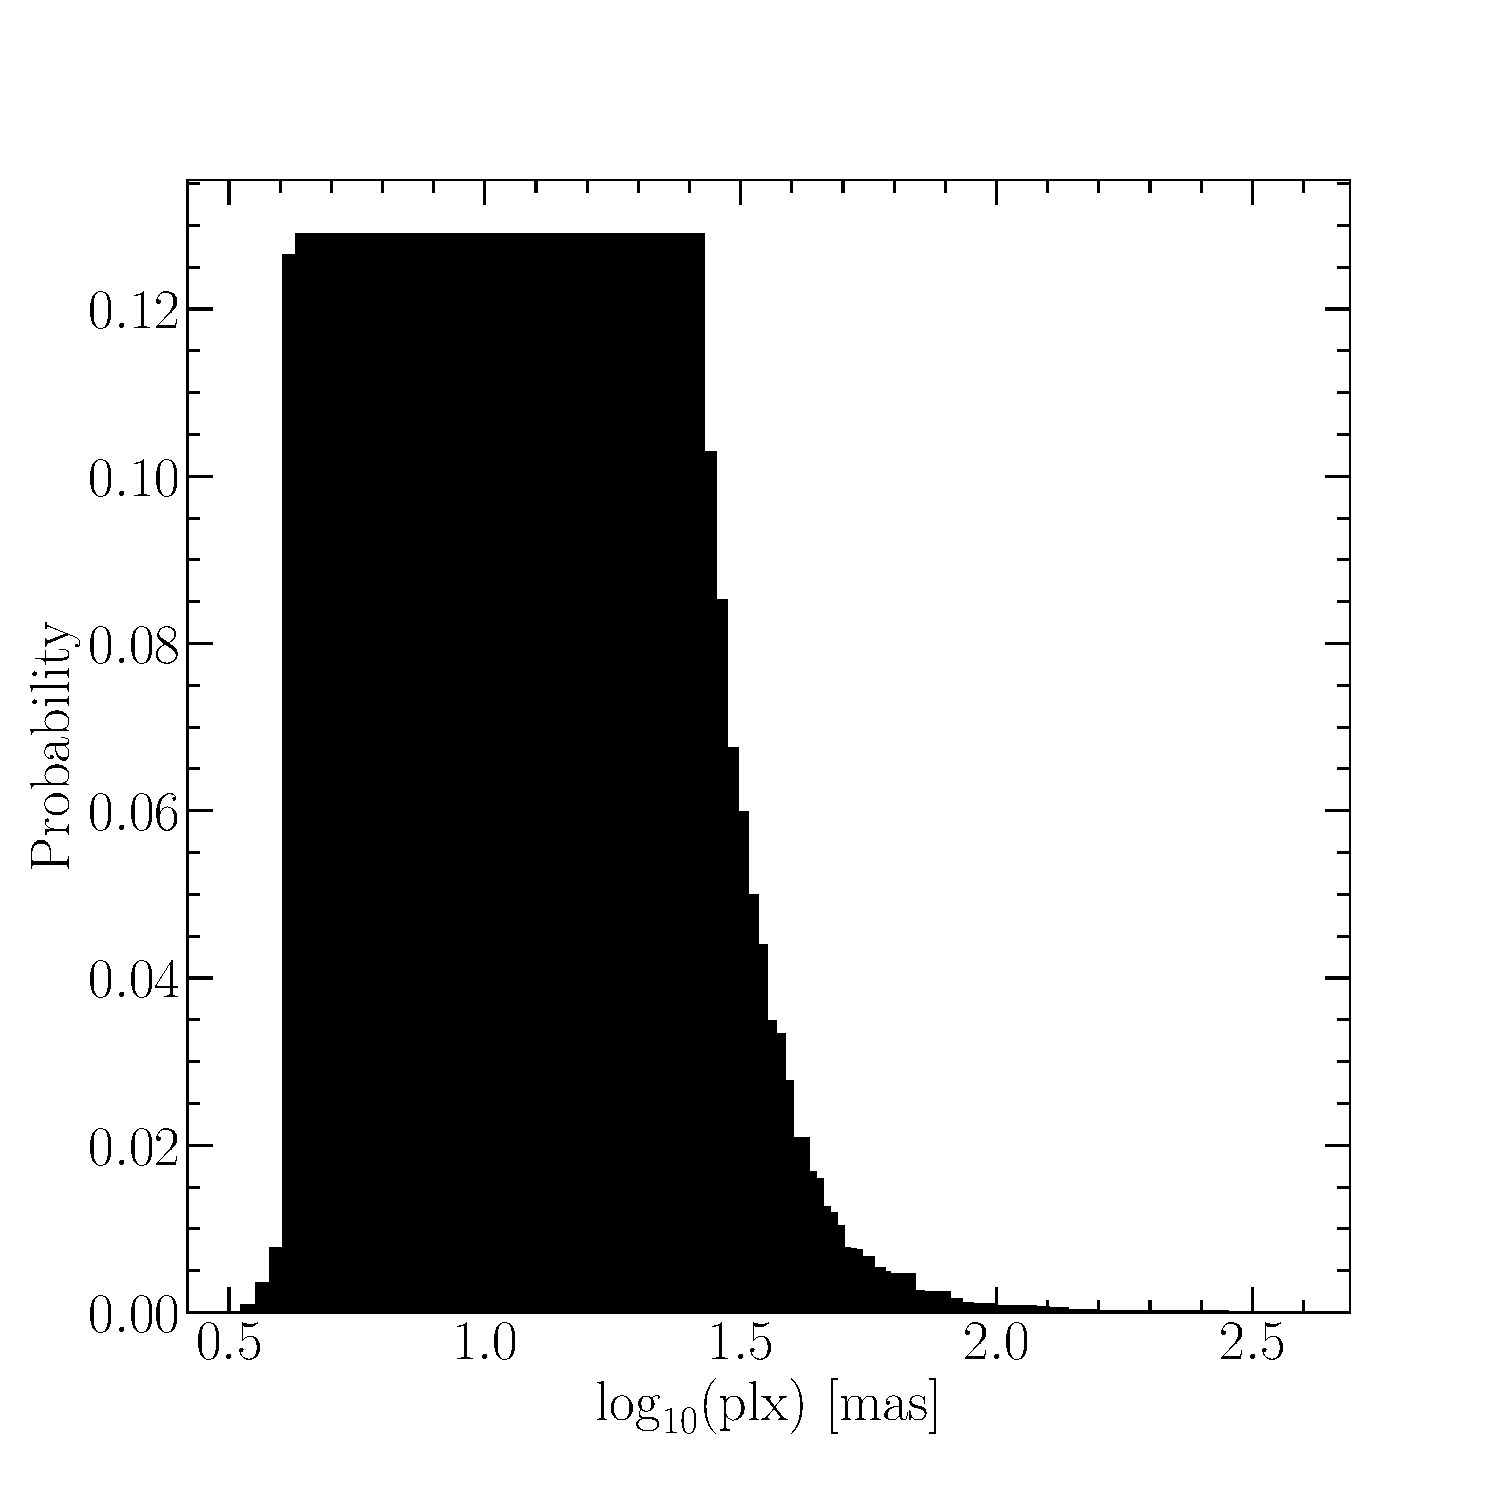
\includegraphics[width=0.45\textwidth]{src/figures/NotebookFigs/pdist.pdf}
	\caption{Probability distribution sampled when assigning true parallaxes to
	synthetic stars. This distribution is built from the GCNS and includes all
	stars with BP-RP colors between 2.3 and 2.9, the same color range
	of the Jao Gap.}
	\label{fig:pdist}
\end{figure}

\begin{enumerate}
	\item Sample from a \citet{Sollima2019} ($0.25 M_{\odot} < M < 1 M_{\odot}$,
		$\alpha=-1.34\pm0.07$) IMF to determine synthetic star mass.
	\item Find the closest model above and below the synthetic star, lineally
		interpolate these models' $T_{eff}$, $\log(g)$, and $\log(L)$ to those
		at the synthetic star mass.
	\item Convert synthetic star $g$, $T_{eff}$, and $Log(L)$ to Gaia G, BP,
		and RP magnitudes using the Gaia (E)DR3 bolometric corrections
		\citep{Creevey2022} along with code obtained thorough personal
		communication with Aaron Dotter \citep{Choi2016}.
	\item Sample from the GCNS parallax distribution (Figure \ref{fig:pdist}),
		limited to stars within the BP-RP color range of 2.3 -- 2.9, to assign
		synthetic star a ``true'' parallax.
	\item Use the true parallax to find an apparent magnitude for each filter.
	\item Evaluate the empirical calibration given in Equation
		\ref{eqn:plxCalib} to find an associated parallax uncertainty. Then
		sample from a normal distribution with a standard deviation equal to
		that uncertainty to adjust the true parallax resulting in an
		``observed'' parallax.
	\item Use the ``observed'' parallax and the apparent magnitude to find an
		``observed'' magnitude.
	\item Fit the empirical calibration given in Equation \ref{eqn:MagCalib} to
		the GCNS and evaluate it to give a magnitude uncertainty scale in each
		band.
	\item Adjust each magnitude by an amount sampled from a normal
		distribution with a standard deviation of the magnitude uncertainty
		scale found in the previous step.
\end{enumerate}

This method then incorporates both photometric and astrometric uncertainties
into our population synthesis. An example 7 Gyr old synthetic populations
using OPAL and OPLIB opacities are presented in Figure
\ref{fig:PopSynthCompareBasic}.

\begin{figure*}
	\centering
	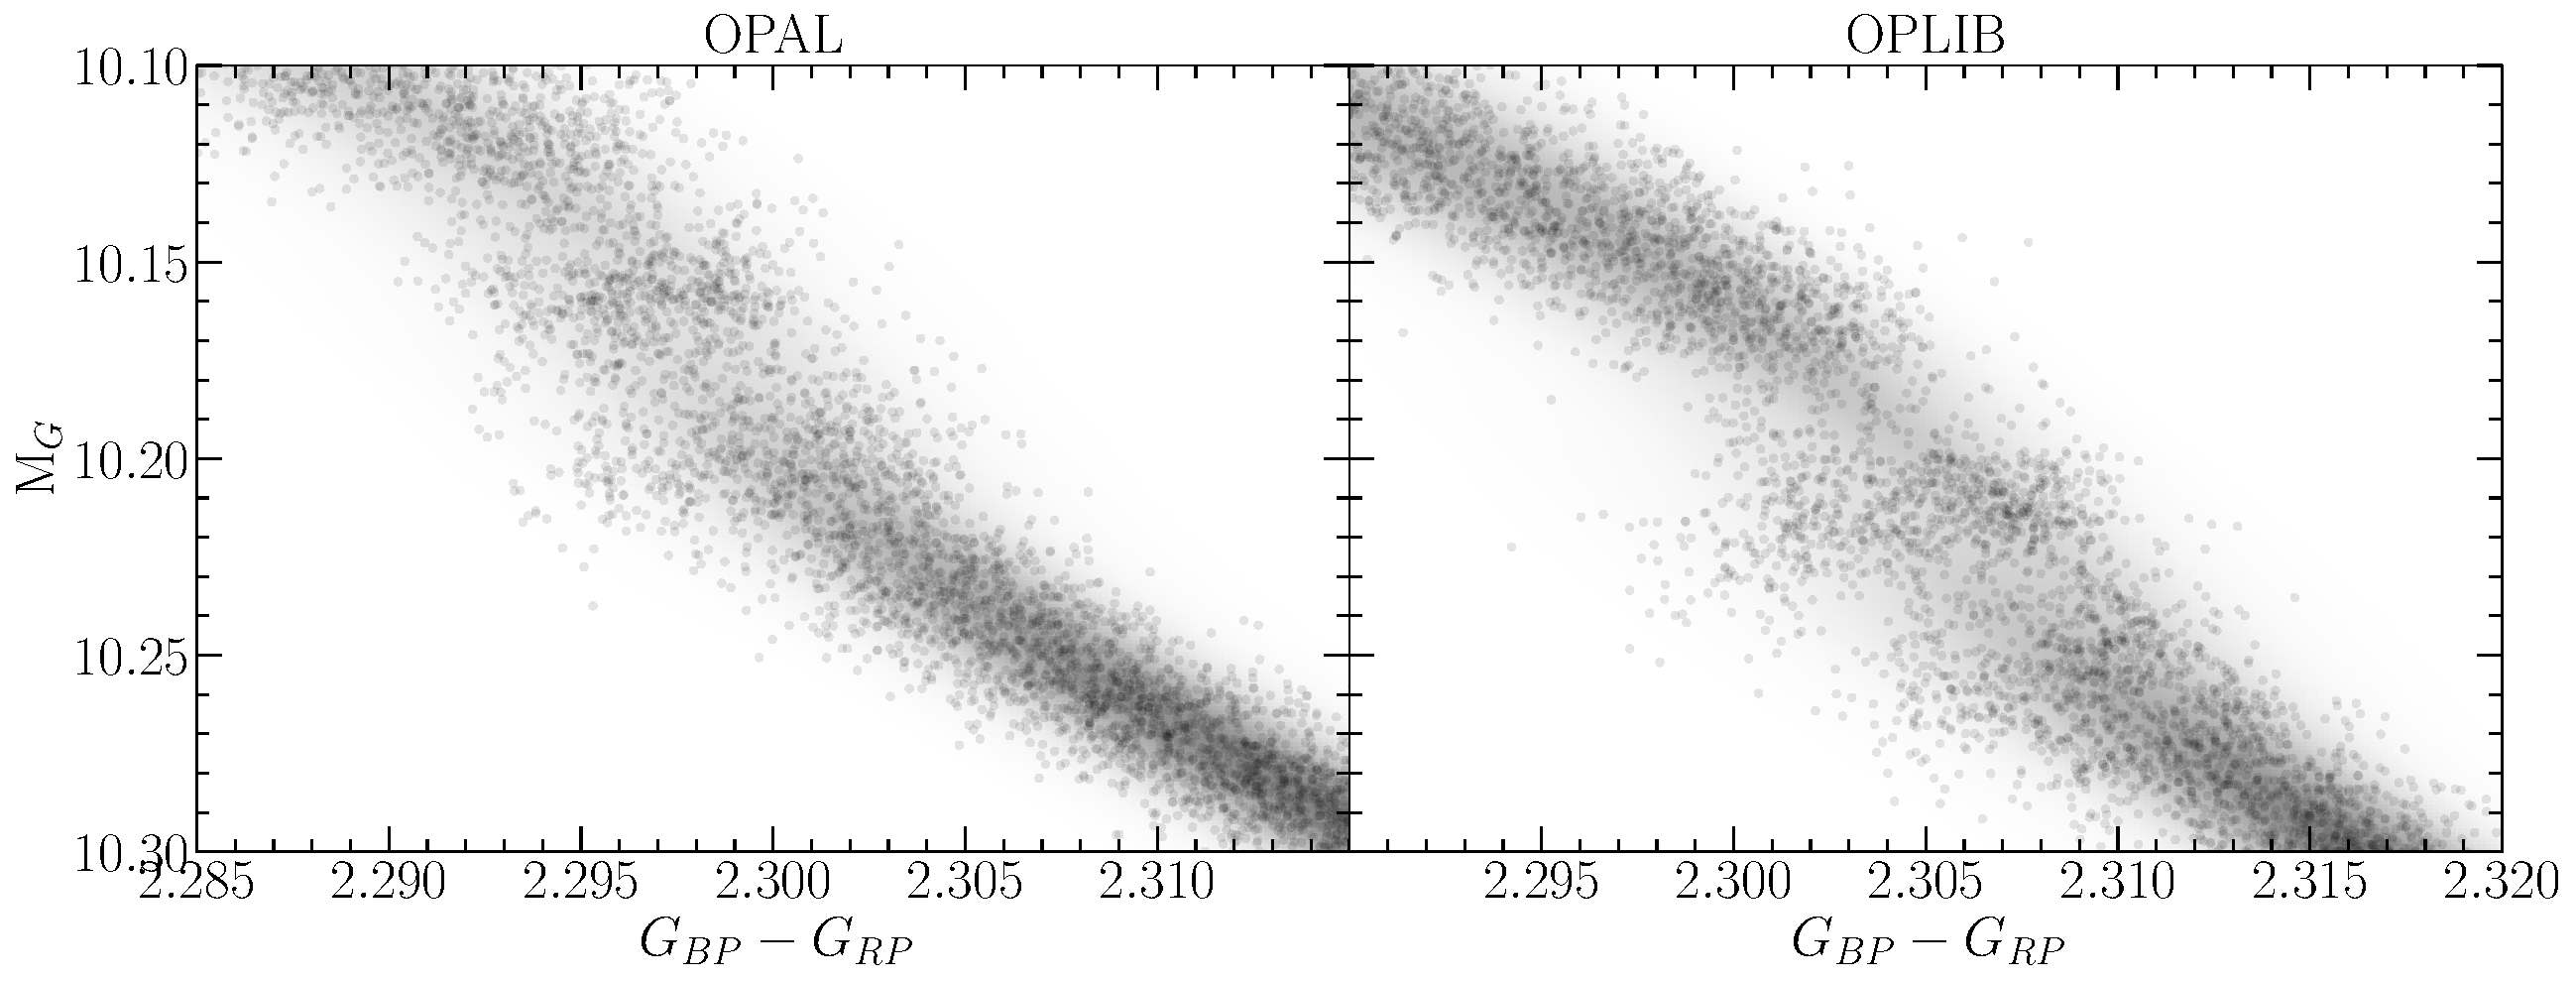
\includegraphics[width=0.85\textwidth]{src/figures/NotebookFigs/OPALOPLIB_popsynth_compare.pdf}
	\caption{Population synthesis results for models evolved with OPAL (left)
	and models evolved with OPLIB (right). A Gaussian kernel-density estimate
	has been overlaid to better highlight the density variations.}
	\label{fig:PopSynthCompareBasic}
\end{figure*}


\section{Results}\label{sec:results}
We quantify the Jao Gap location along the magnitude axis by first subsampling
our synthetic populations, finding the linear number density along the
magnitude axis of each subsample, averaging these linear number density and
extracting peaks from this above a prominence threshold.w Once we have the peak
location we fit a gaussian to a window centered at the peak giving both an
estimate of the gap location and the gap width. Figure \ref{fig:JaoGapLocator}
shows this fit for both OPAL and OPLIB populations.

\begin{table}
	\centering
	\begin{tabular}{c | c c}
		\hline
		Model & Location & Prominence \\
		\hline
		\hline
		OPAL & 10.15864 & 0.19501 \\
		OPLIB 1 & 10.17813 & 0.26055 \\
		OPLIB 2 & 10.21313 & 0.46898
	\end{tabular}
	\caption{Locations identified as potential gaps.}
	\label{tab:GapLocation}
\end{table}

Our gap identification method finds two potential gaps in the OPLIB (Table
\ref{tab:GapLocation}) data while only finding one in the OPAL dataset. This
apparent discrepancy is not due to a fundamental structural difference between
the OPAL and OPLIB opacity tables; rather, it is attributable to the the
phasing of the periodic luminosity variations seen accorss mass in Figures
\ref{fig:OPALPunchIn} and \ref{fig:OPLIBPunchIn} and whether or not the
injected noise smears all of these together into one gap or two gaps.
{\color{red} [Run a test where you manually shift the OPAL data to the same
phase as the OPLIB data to show that this has the effect of making two gaps
show up]}.

\begin{figure}
	\centering
	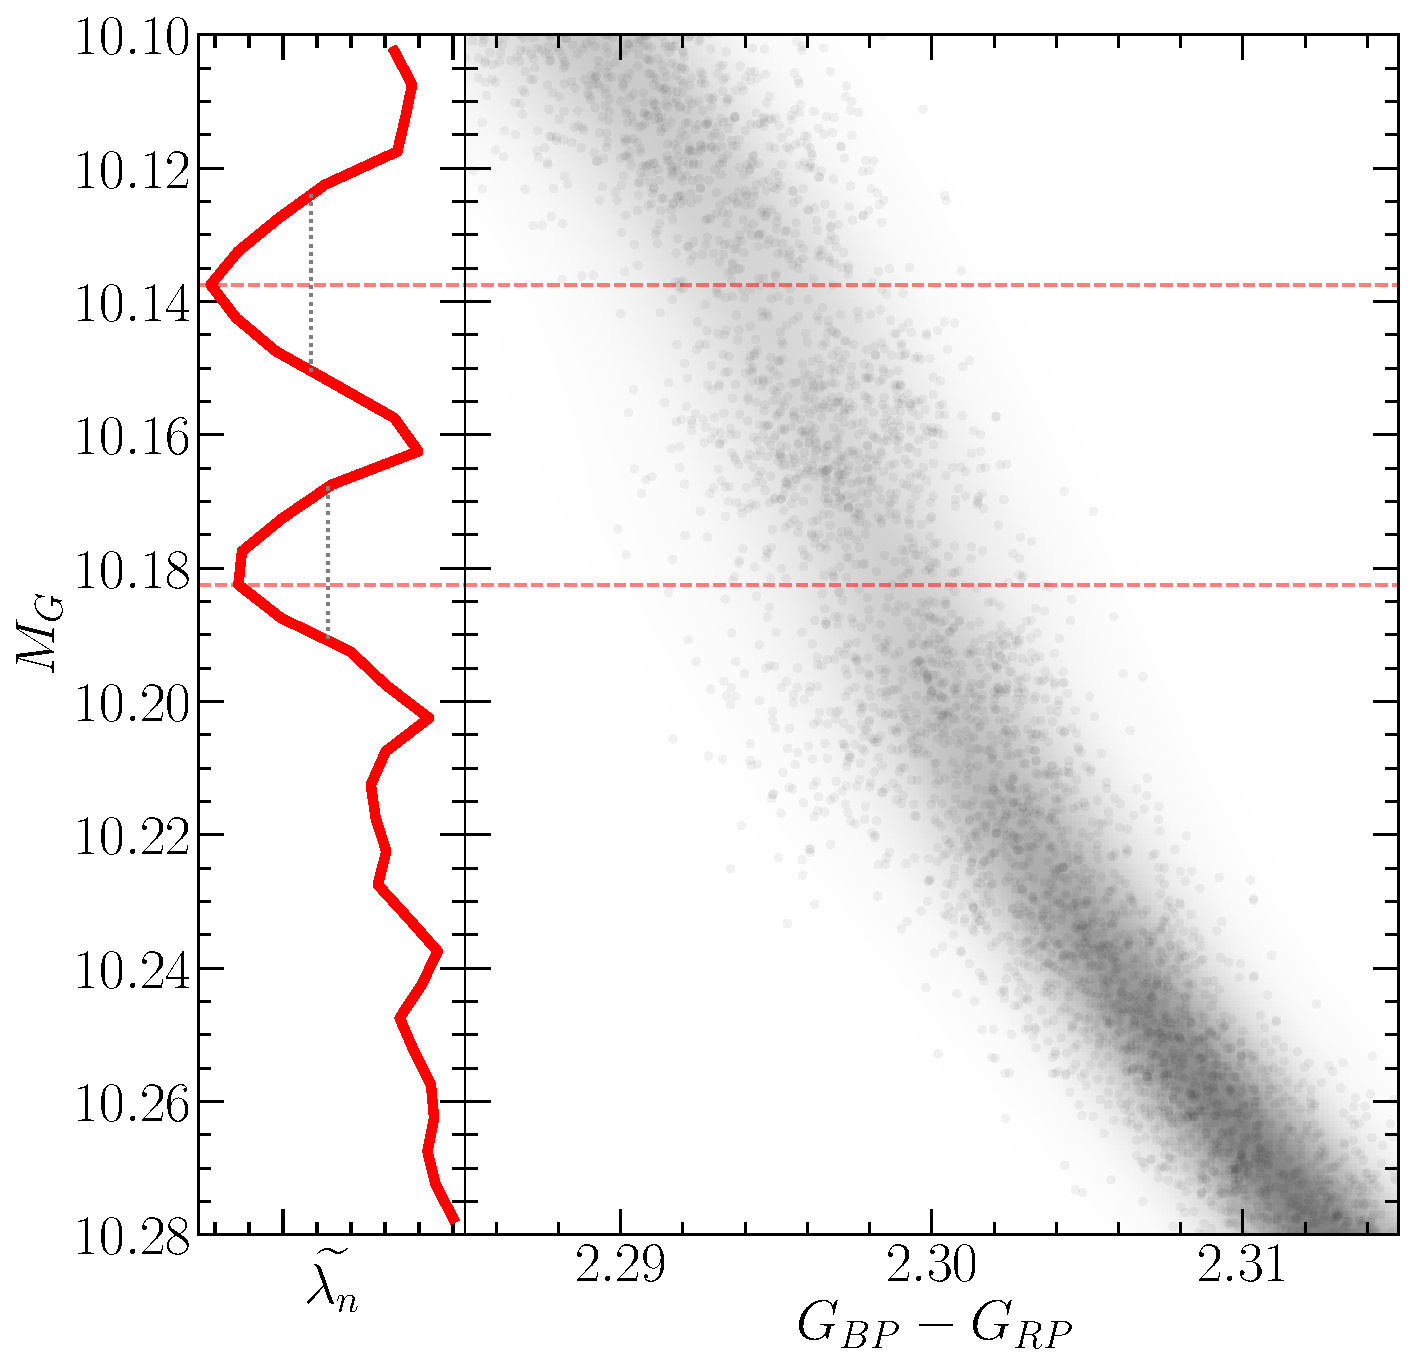
\includegraphics[width=0.45\textwidth]{src/figures/NotebookFigs/OPAL_Jao_locator.png}
	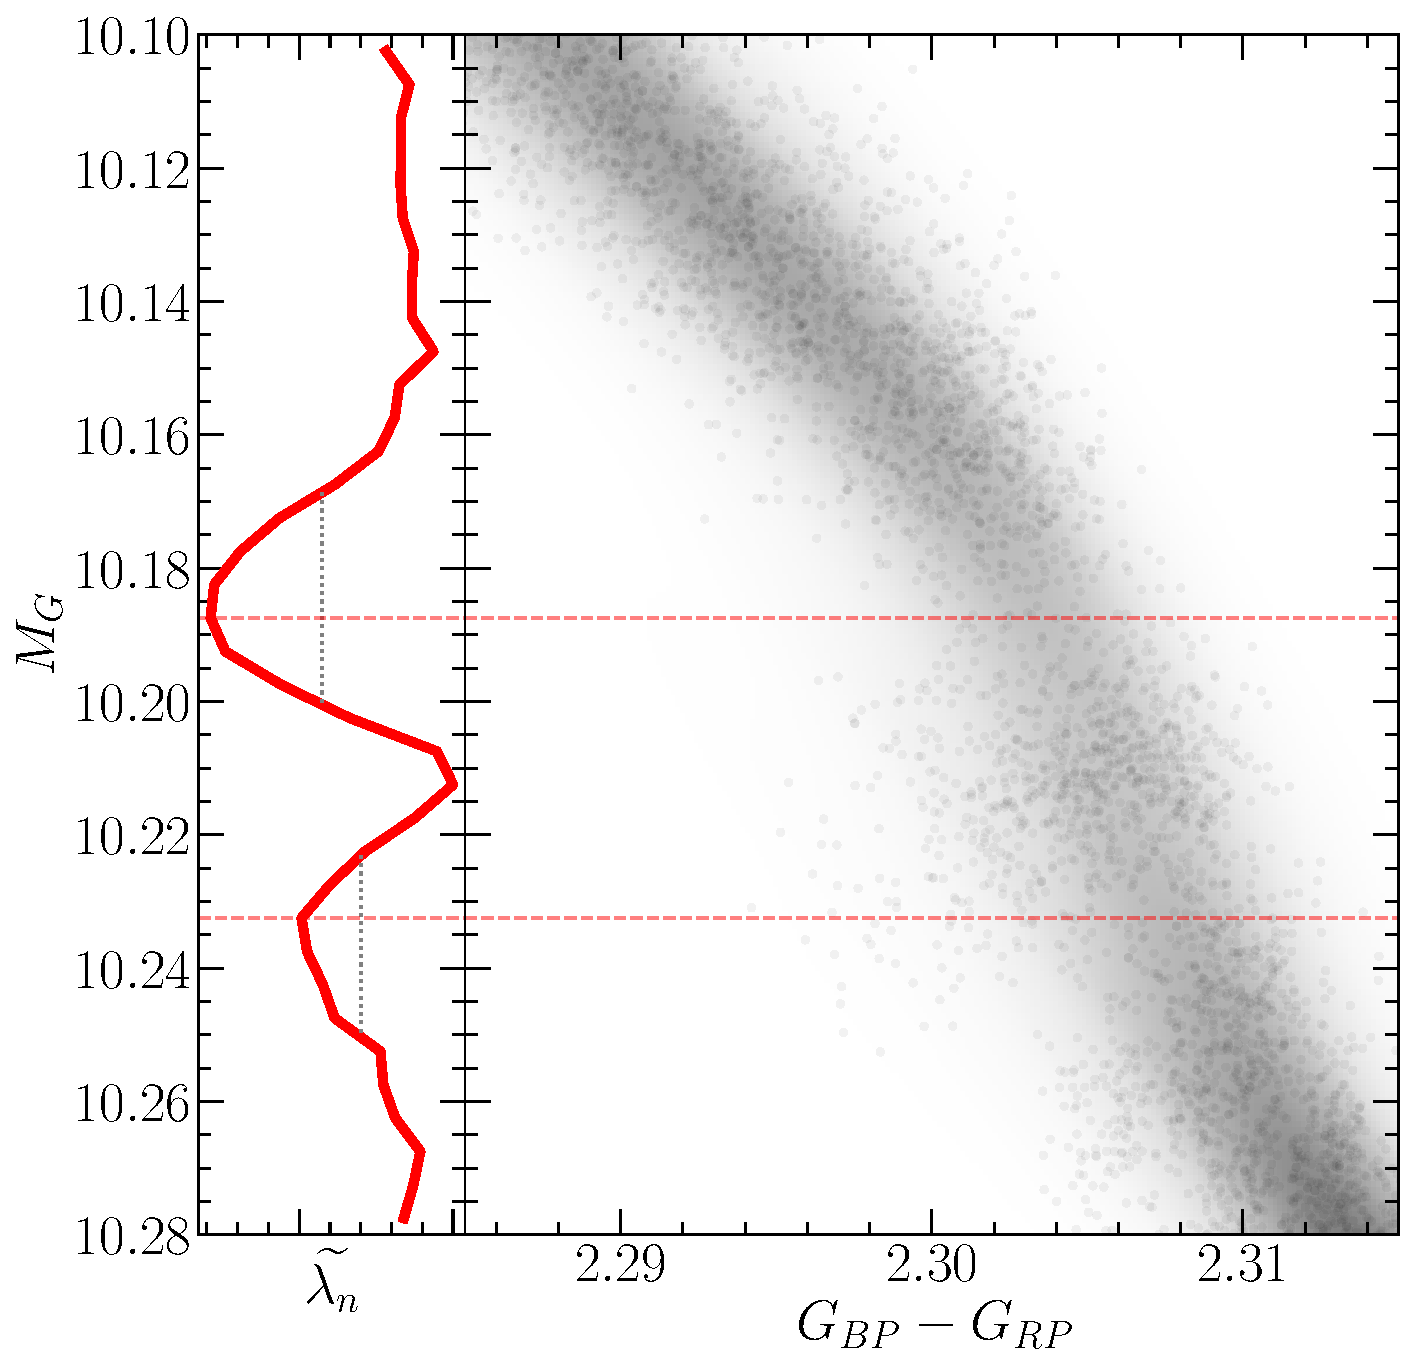
\includegraphics[width=0.45\textwidth]{src/figures/NotebookFigs/OPLIB_Jao_locator.png}
	\caption{(right panels) OPAL (top) and OPLIB (bottom) synthetic
	populations. (left panels) Normalized linear number density along the
	magnitude axis. A dashed line has been extended from the peak through both
	panels to make clear where the Identified Jao Gap location is wrt. to the
	population. }
	\label{fig:JaoGapLocator}
\end{figure}

Both gaps identified in the OPLIB sample are at fainter magnitudes than the gap
identified in the OPAL sample. This implies that in the OPLIB sample the
convective mixing events which drive the kissing instability should happen more
regularlry and therefore also start earlier in the models evolution. This is
because each mixing event serves to interupt the ``standard'' luminosity
evolution of a stellar model, kicking its luminosity back down to what it would
have been a few Gyrs earlier instead of allowing it to slowly increase. Looking
at the interior physics of one OPAL and one OPLIB model shows that this shorter
duration between mixing events is in fact seen (Figure {\color{red} [PUT
KIPPENHAN DIAGRM HERE]}.

The slightly lower opacities charectaristic to OPLIB serve to shallow the
radiative temperature gradient, $\nabla T_{rad}$; however, as the adiabatic
temperature gradient remains essentially unchanged, a larger interior radius of
the model will remain unstable to convection {\color{red}[CHECK IF THIS OR IF
RADIATIVE ZONE MOVING IN]}. This larger convective zone and therefore smaller
radiative zone is in line with the behavior of the models presentd here. We see
that OPLIB models undergo convective mixing events earlier in their evolution
than OPAL models (Figure \ref{fig:OPALOPLIB3He} implying that the inner
convective zone did not have to expand as much to meet the outer convective
zone. 

\begin{figure}
	\centering
	\includegraphics[width=0.45\textwidth]{src/figures/NotebookFigs/3HeOPAL_OPLIB.pdf}
	\caption{Core $^{3}$He mass fraction for a model evolved with OPAL and a
	model evolved with OPLIB within the Jao Gap's mass range. Note how the
	OPLIB model undergoes the mixing event earlier in its evolution than the
	OPAL model does.}
	\label{fig:OPALOPLIB3He}
\end{figure}

{\color{red} Then compare the results to observations, comment on which one
matches observations better and also how confident we can be about that}

{\color{red} Comment on if the shift in the gap location is larger or smaller
than the size o fthe gap or the shift due to other effects such as variations
in age or composition, i.e is it Significant enough to matter}

{\color{red} comment on why the gap shifts in the manner which it does, i.e the
opacities are lower. Show how for a constant opacity table increasing the
metallicity (which will also change the opacity) affetcs the gap location)}


\section{Conclusion}\label{sec:conclusion}
The Jao Gap provides an intriguing probe into the interior physics of M Dwarfs
stars where traditional methods of studying interiors break down. However,
before detailed physics may be inferred it is essential to have models which
are well matched to observations. Here we investigate whether the OPLIB opacity
tables reproduce the Jao Gap location and structure more accurately than the
widely used OPAL opacity tables. We find that while the OPLIB tables do shift
the Jao Gap location more in line with observations, by approximately 0.05
magnitudes, the shift is small enough that it is likely not distinguishable
from noise due to population age and chemical variation. Moreover, we do not
find that the OPLIB opacity tables help in reproducing the wedge shape of the
observed Gap.


\appendix

\section{Interpolating $\rho \rightarrow $ R}\label{apx:interp}
OPLIB reports $\kappa_{R}$ as a function of mass density, temperature in keV,
and composition. DSEP uses tables where opacity is given as a
function of temperature in Kelvin, $R$, and composition. The conversion from
temperature in keV to Kelvin is trivial
\begin{align}
	T_{K} = T_{keV} * 11604525.0061657
\end{align}
However, the conversion from mass density to $R$ is more involved. Because $R$ is
coupled with both mass density and temperature there there is no way to
directly convert tabulated values of opacity reported in the OPLIB tables to
their equivalents in $R$ space. Instead we must rotate the tables,
interpolating $\kappa_{R}(\rho,T_{eff}) \rightarrow \kappa_{R}(R,T_{eff})$. 

To preform this rotation we use the \texttt{interp2d} function within
\texttt{scipy}'s \texttt{interpolate} \citep{2020SciPy-NMeth} module to
construct a cubic bivariate B-spline \citep{Dierckx1981} interpolating function
$s$, with a smoothing factor of 0, representing the surface $\kappa_{R}(\rho,
T_{eff})$. For each $R^{i}$ and $T^{j}_{eff}$ which DSEP expects
high-temperature opacities to be reported for, we evaluate Equation
\ref{eqn:Req} to find $\rho^{ij} = \rho(T^{j}_{eff},R^{i})$.  Opacities in
$T_{eff}$, $R$ space are then inferred as $\kappa^{ij}_{R}(R^{i},T^{j}_{eff}) =
s(\rho^{ij}, T^{j}_{eff})$. 

As first-order validation of this interpolation scheme we can preform a similar
interpolation in the opposite direction, rotating the tables back to
$\kappa_{R}(\rho, T_{eff})$ and then comparing the initial, ``raw'', opacities
to those which have gone through the interpolations process. Figure
\ref{fig:fracdiff} shows the fractional difference between the raw opacities
and a set which have gone through this double interpolation. The red line
denotes $\log(R)=-1.5$ where models will tend to sit for much of their radius.
Along the $\log(R)=-1.5$ line the mean fractional difference is $\langle \delta
\rangle = 0.006$ with an uncertainty of $\sigma_{\langle\delta\rangle} =
0.009$. One point of note is that, because the initial rotation into $\log(R)$
space also reduces the domain of the opacity function interpolation-edge
effects which we avoid initially by extending the domain past what DSEP needs
cannot be avoided when interpolating back into $\rho$ space. 

\begin{figure}
	\centering
	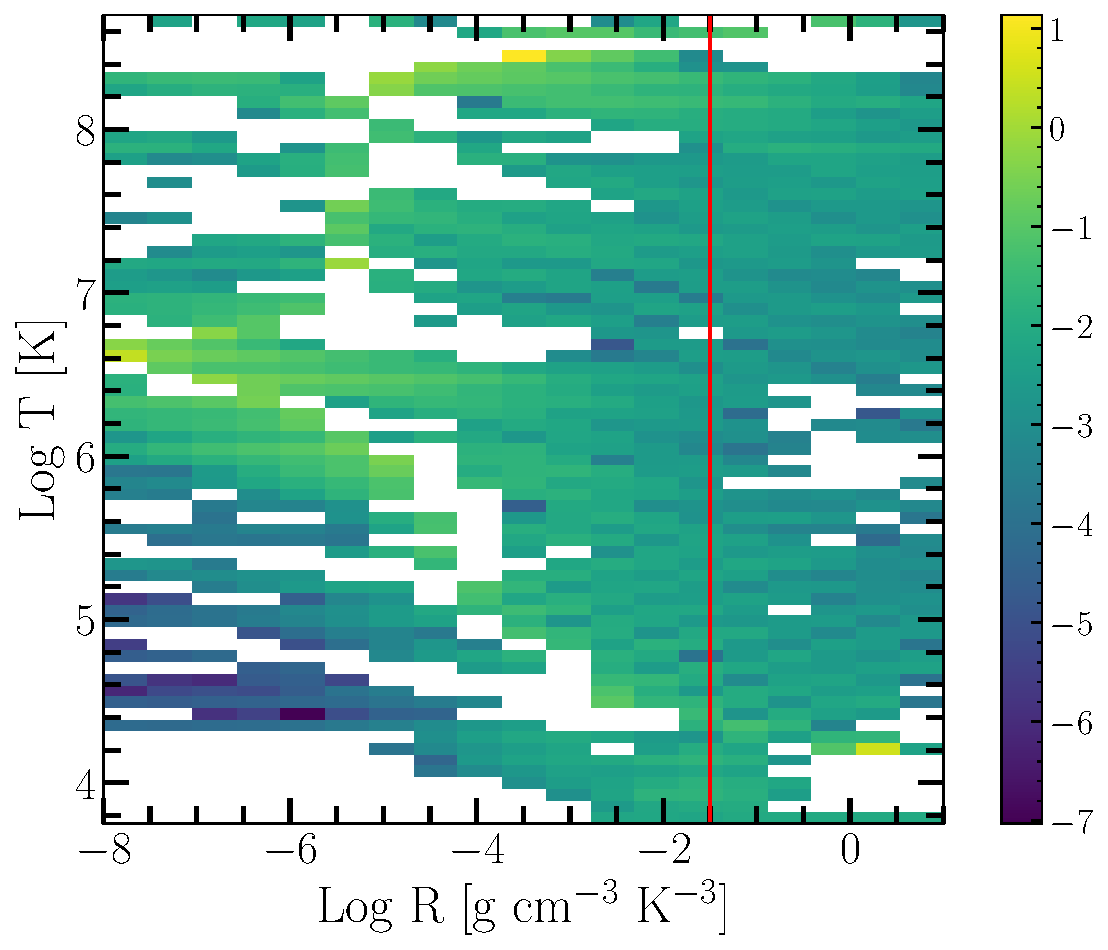
\includegraphics[width=0.45\textwidth]{src/figures/FractionalDifference.pdf}
	\caption{Log Fractional Difference between opacities in $\kappa_{R}(\rho,
	T_{eff})$ space directly queried from the OPLIB web-form and those which
	have been interpolated into $\log(R)$ space and back. Note that, due to the
	temperature grid DSEP uses not aligning perfectly which the temperature
	grid OPLIB uses there may be edge effects where the interpolation is poorly
	constrained. The red line corresponds to $\log(R) = -1.5$ where much of a
	stellar model's radius exists.}
	\label{fig:fracdiff}
\end{figure}



\bibliography{src/bib/ms}{}
\bibliographystyle{aasjournal}


\end{document}

